\section{Introduction}
Once the first version of the automated pipeline was built, it could begin to be used it to reduce the ULTRACAM archive in order to evaluate how effective it was. The first aspect to investigate was whether the photometry the pipeline produced was of sufficient quality to allow researchers to view light-curves that clearly demonstrate astronomical phenomena occuring in the data. Reductions of runs of some well known objects were inspected and compared the photometry produced by the traditional pipeline. The effectiveness of the web interface as a method of discovering new variable objects was tested by visual inspection the output of the automated pipeline and searching for variability in the light-curves. The expectation was that it should be easy to identify the intended target of each run even if the field contained many objects, since the target would likely reveal itself through its variability. Finally, the pipeline was instructued to process all of the ULTRACAM archive to evaluate if it was robust enough to reduce the full set of the data despite the diversity of the input. 

\section{Quality of the photometry}
The purpose of this project was to establish a process for automatically reducing the light-curves for all objects in the data archive rather than trying to produce accurate and well-calibrated measurements. The diverse nature of the dataset means that it is not trivial to write an automated algorithm that can perform fully-calibrated measurements. The automated pipeline lacks the ability to correctly identify the appropriate bias readings, flat-fields and standard stars that should be used for photometric calibration. Therefore, these steps are skipped altogether. The magnitudes and flux counts produced by the automated pipeline are not calibrated and will differ from their true values by arbitrary offsets. 

\begin{figure}
\centering
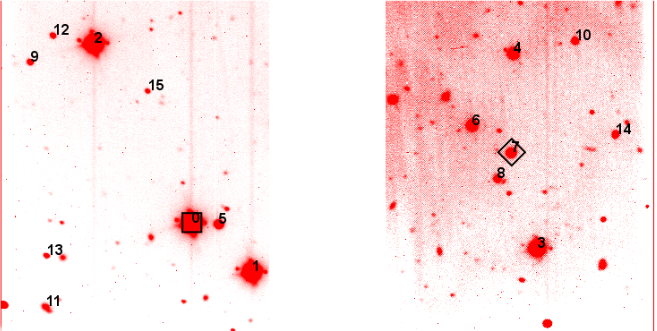
\includegraphics[width=120mm]{images/2013-07-13-run111-r-withlabels.png}
\caption{Snapshot taken from the automated pipeline browser for 2013-07-13/run111. The target, {NN Ser} is labeled `7' and the object we have used as the comparison is  '0' in the image. This is a stacked image from the red CCD taken through the Sloan 'i' filter. }
\label{fig:nnserfield}
\end{figure}

Since the ULTRACAM has a well-established data reduction pipeline, it is useful to compare the results of this pipeline with the new, automated one built in this project. As mentioned above, the automated pipeline does not perform calibrated photometry, but we can still compare the non-calibrated photometry to get an estimate of how well our new pipeline performs.

In order to do this, I chose a run of a target object that has often been observed with ULTRACAM. The object is NN Ser, a white-dwarf, M-dwarf eclipsing binary. The specific run chosen was \emph{2013-07-13/run111}. Producing the photometry using the automated pipeline on this run is achieved by simply typing: \texttt{runbuilder.py 2013-07-13/run111} on the command line. Please refer to the user manual in appendix \ref{chap:usermanual} for instructions on how to install and run the pipeline.  The reduction takes about 5 minutes to process when running on a standard desktop machine in the University of Warwick Astronomy department. The output of this reduction can be seen at \url{http://deneb.astro.warwick.ac.uk/phrnaw/sitedev/2013-07-13/run111.html}. I also reduced the same run with the traditional pipeline. In both cases I produced light-curves by plotting the relative flux of the target relative to the comparison. Figures \ref{fig:comparepipelines_r} to \ref{fig:comparepipelines_zoom_b} show plots of the results of the automated pipeline together with the traditional pipeline (with a small offset applied to separate the data points). Inspections of these plots show that they produce consistent results. The pipelines seem to have similar RMS scatter and show the same trends. Closer inspection reveals that outlying data points usually occur concurrently,  demonstrating that the systematic differences between the two approaches are smaller than the intrinsic errors in the measurements. 

\begin{figure}
\centering
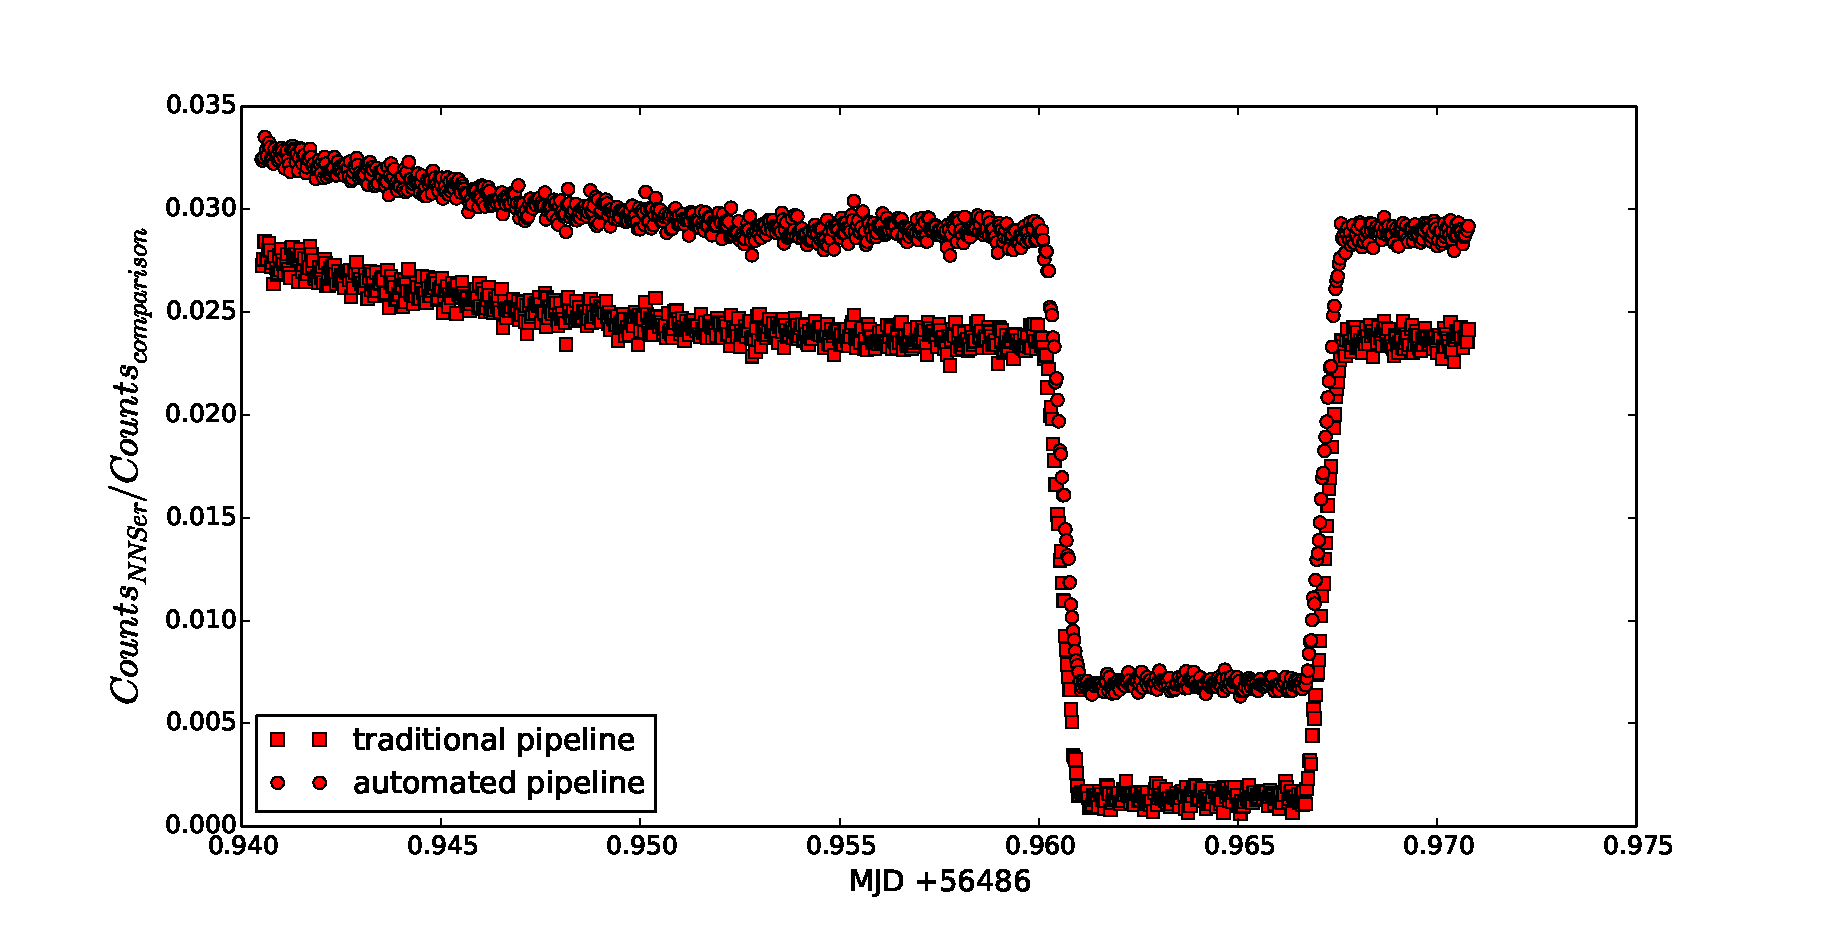
\includegraphics[width=140mm]{images/nn_ser_compare_r.eps}
\caption{Comparison of the light-curves for NN Ser in the Sloan i filter. Square data points were generated by the traditional pipeline and circles by the automated pipeline. The vertical offset applied to the circles is 0.0054. }
\label{fig:comparepipelines_r}
\end{figure}

\begin{figure}
\centering
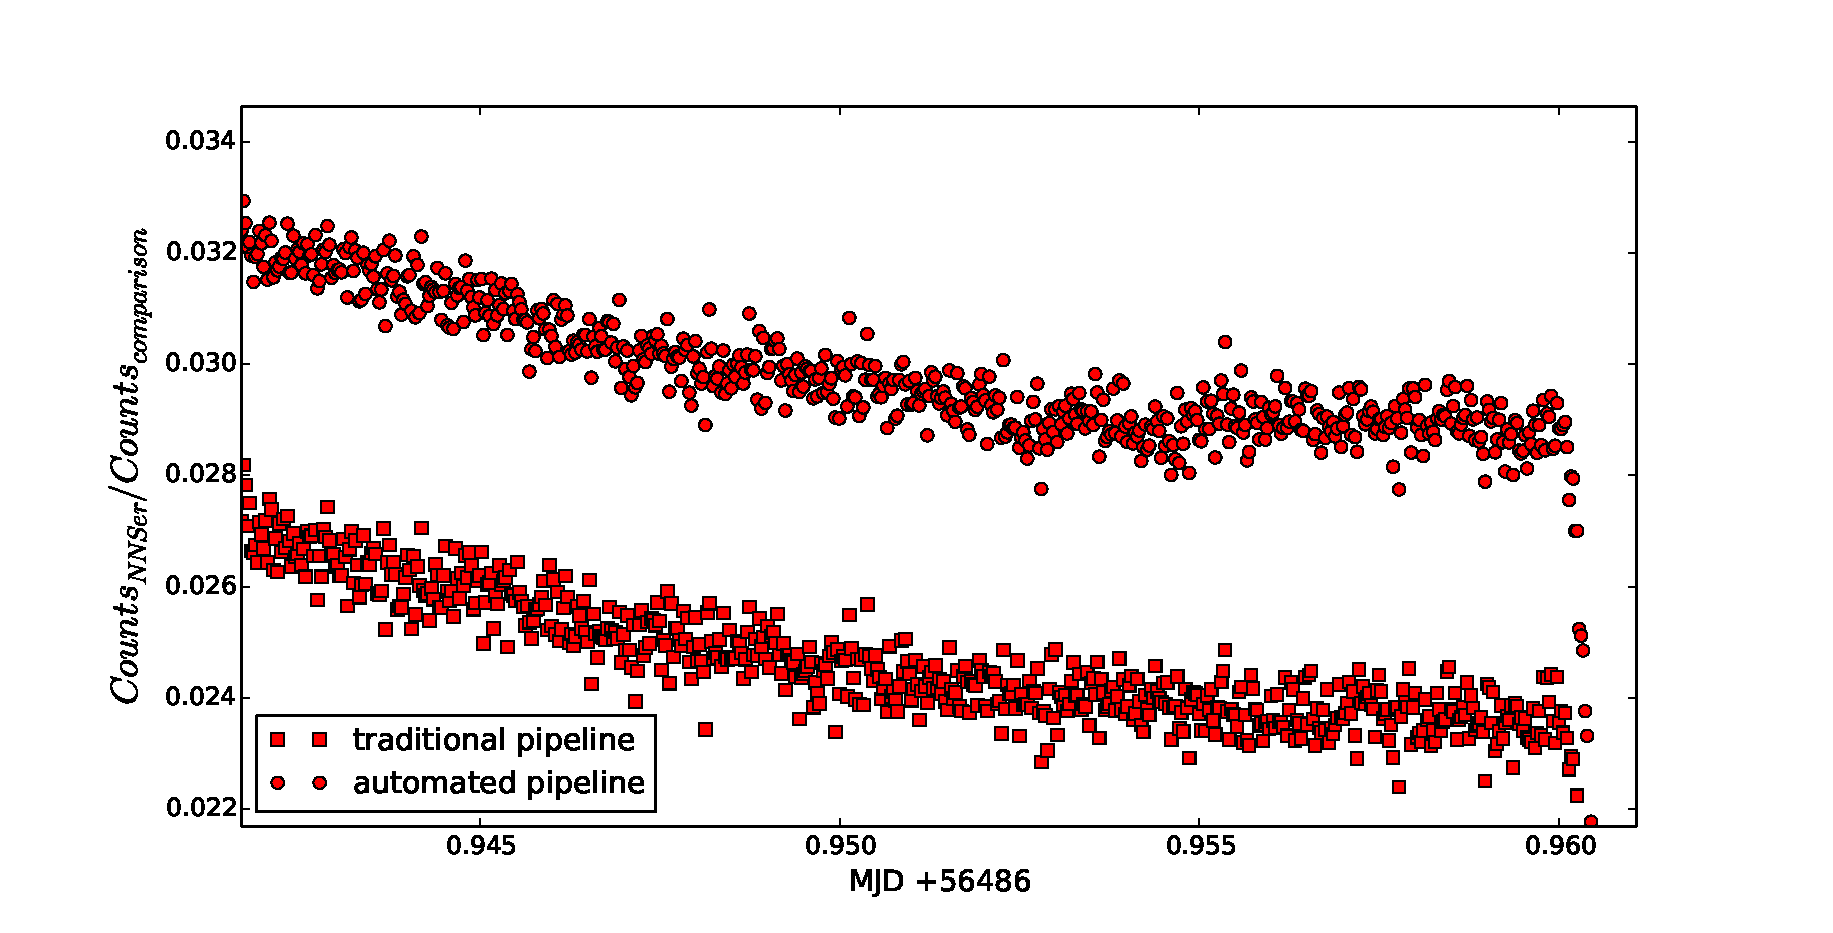
\includegraphics[width=140mm]{images/nn_ser_compare_zoom_r.eps}
\caption{A closer look at the comparison of the light-curves for NN Ser in the Sloan i filter, from the start of the run to the beginning of the eclipse ingress. Square data points were generated by the traditional pipeline and circles by the automated pipeline. The vertical offset applied to the circles is 0.0054. }
\label{fig:comparepipelines_zoom_r}
\end{figure}

\begin{figure}
\centering
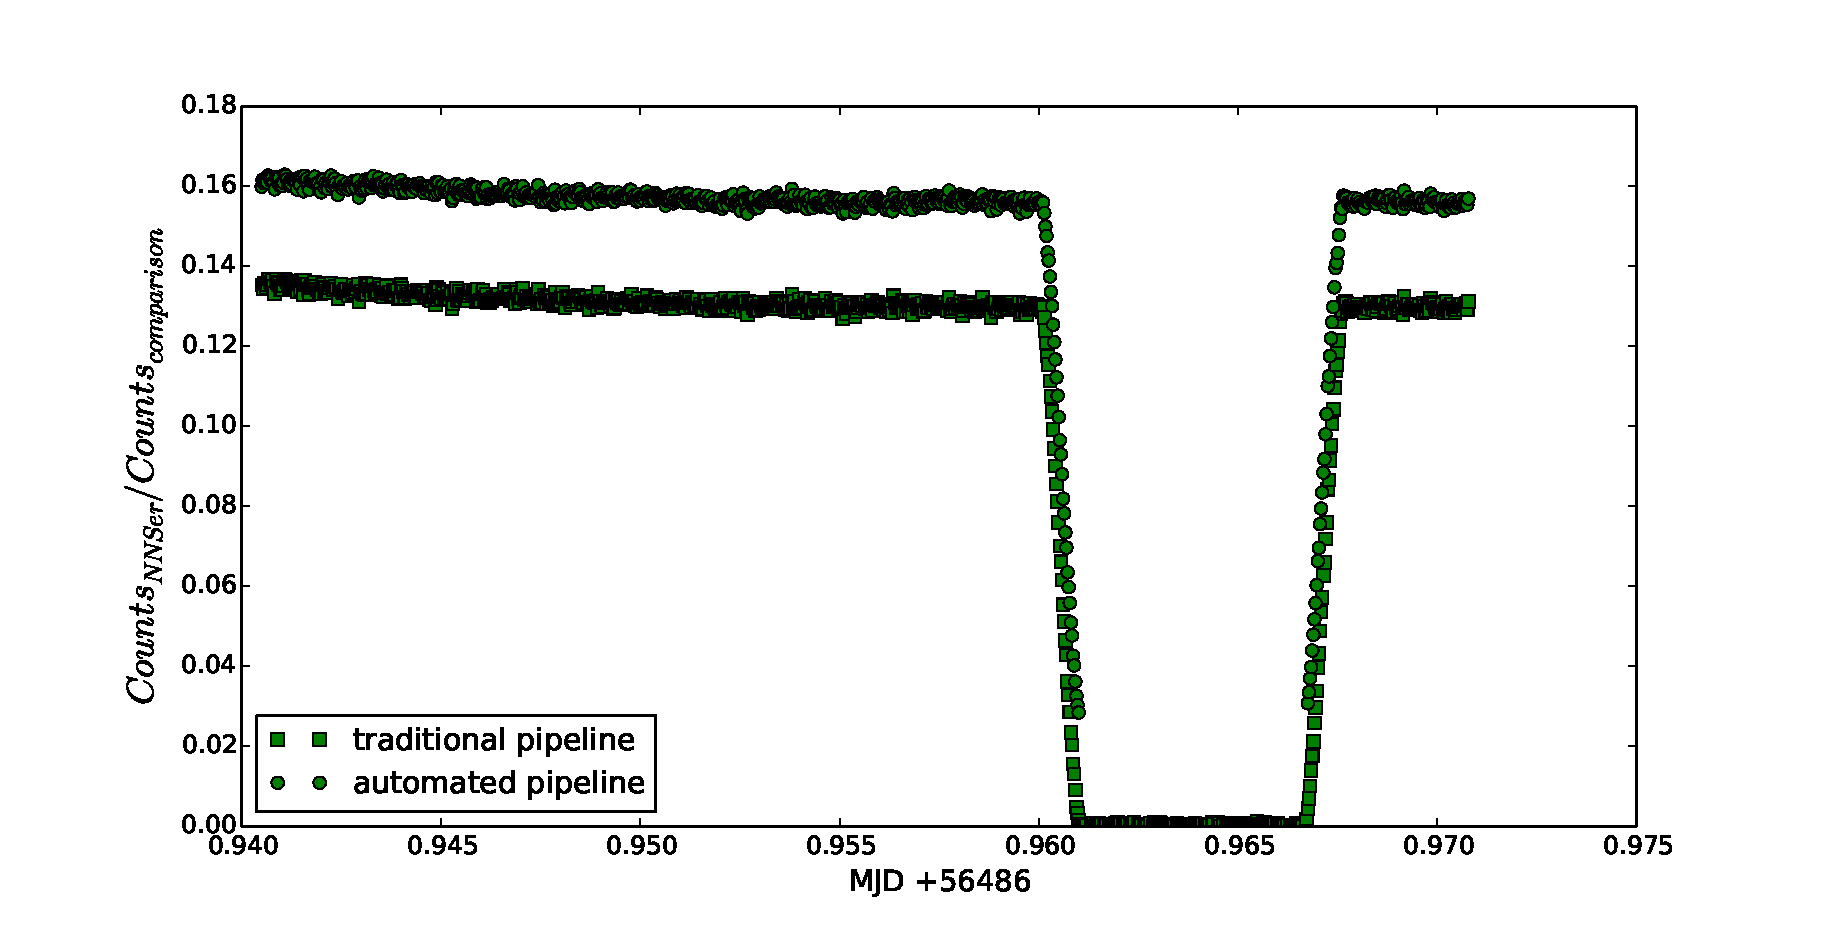
\includegraphics[width=140mm]{images/nn_ser_compare_g.eps}
\caption{Comparison of the light-curves for NN Ser in the Sloan g filter. Square data points were generated by the traditional pipeline and circles by the automated pipeline. The vertical offset applied to the circles is 0.027. Note that the automated pipeline has no data for the duration of eclipse totality. We discuss the reason for this in the text.}
\label{fig:comparepipelines_g}
\end{figure}

\begin{figure}
\centering
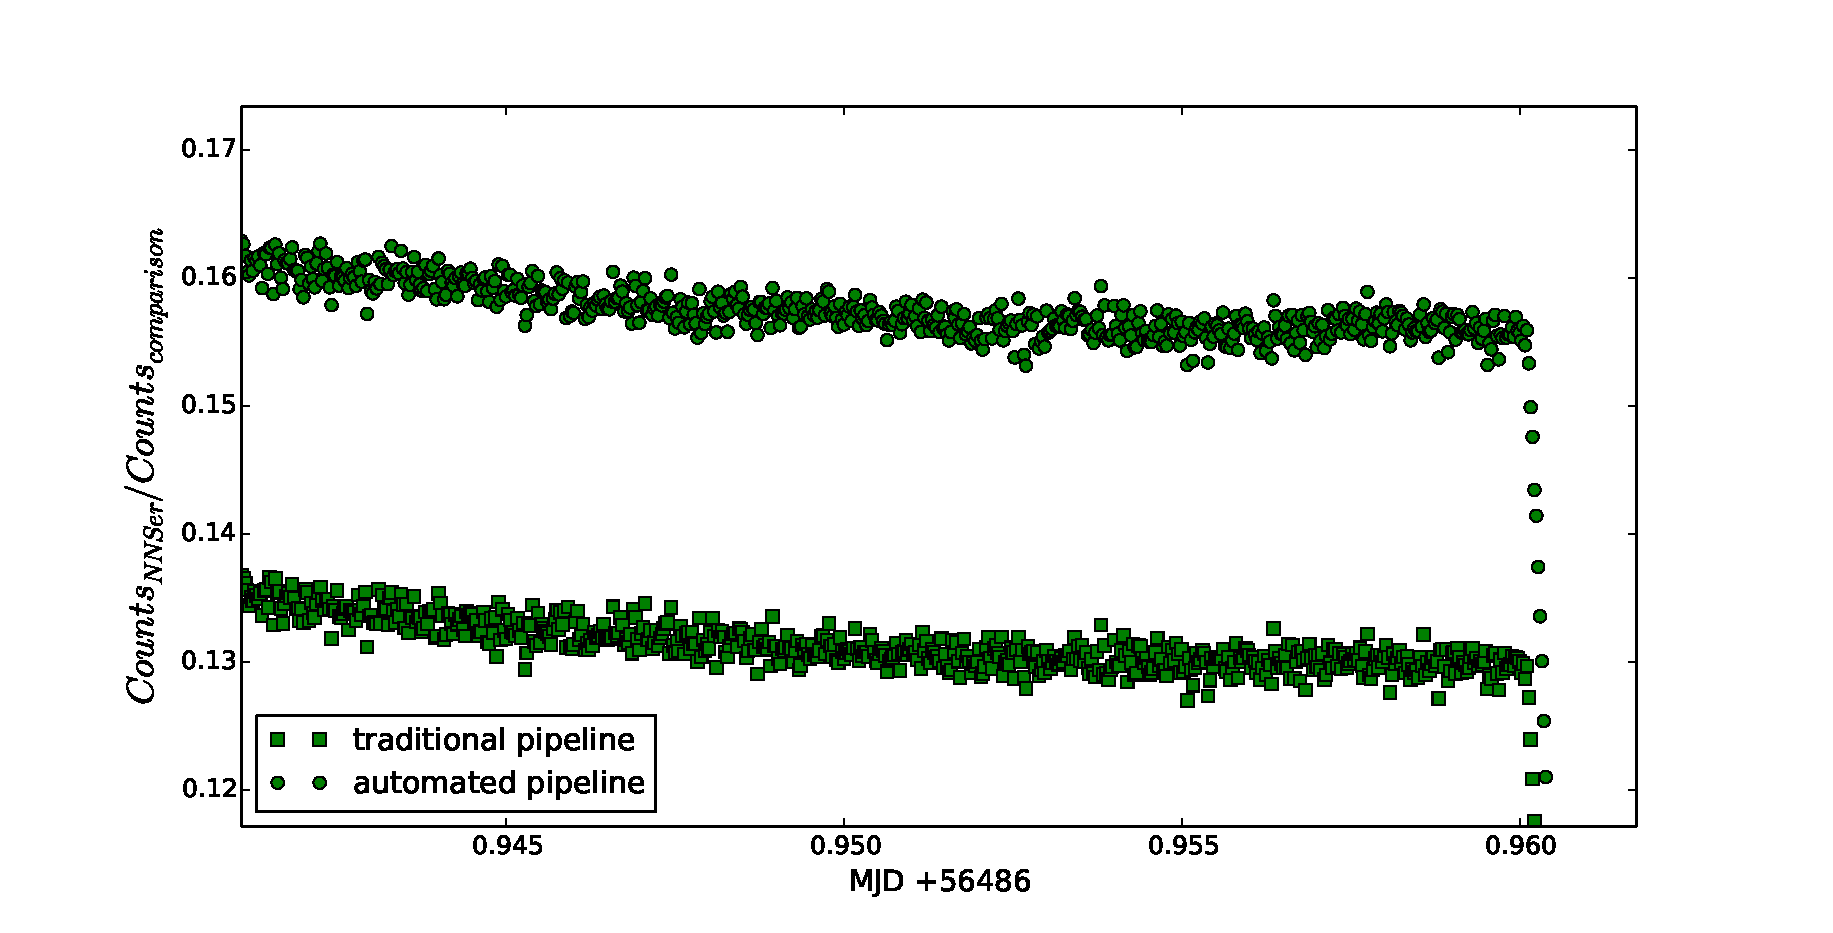
\includegraphics[width=140mm]{images/nn_ser_compare_zoom_g.eps}
\caption{A closer look at the comparison of the light-curves for NN Ser in the Sloan g filter, from the start of the run to the beginning of the eclipse ingress. Square data points were generated by the traditional pipeline and circles by the automated pipeline. The vertical offset applied to the circles is 0.027. }
\label{fig:comparepipelines_zoom_g}
\end{figure}

\begin{figure}
\centering
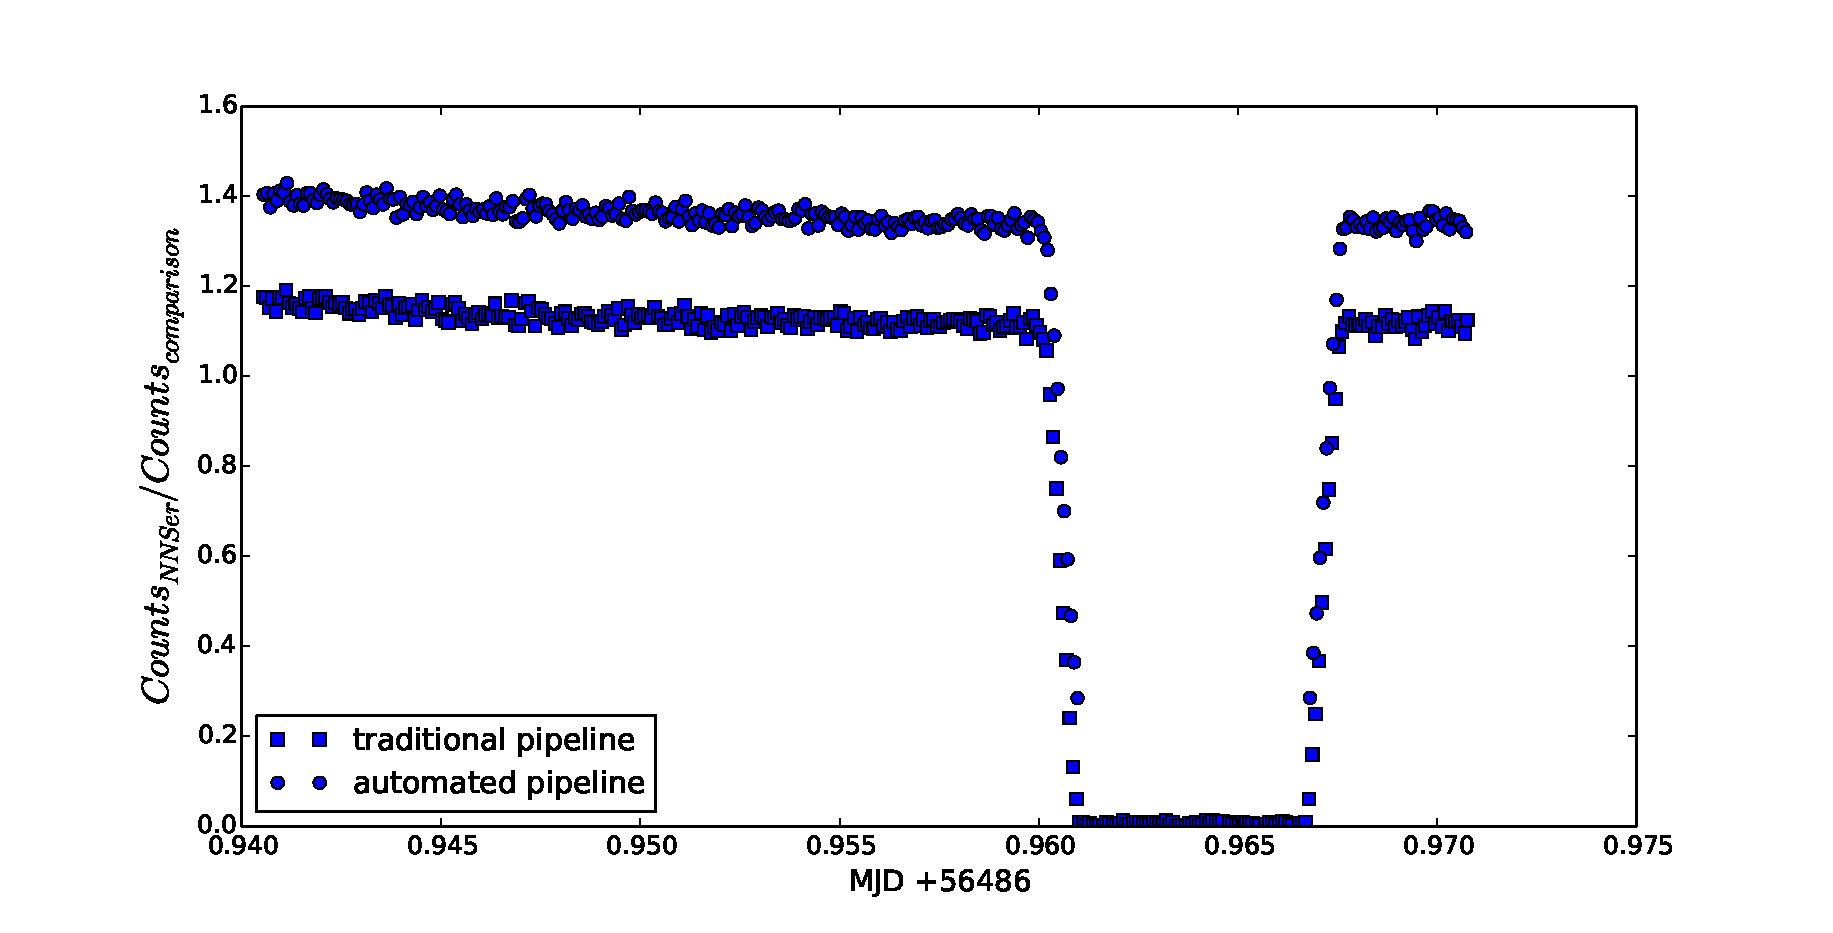
\includegraphics[width=140mm]{images/nn_ser_compare_b.eps}
\caption{Comparison of the light-curves for NN Ser in the Sloan u filter. Square data points were generated by the traditional pipeline and circles by the automated pipeline. The vertical offset applied to the circles is 0.23. Note that the automated pipeline has no data for the duration of eclipse totality. We discuss the reason for this in the text.}
\label{fig:comparepipelines_b}
\end{figure}

\begin{figure}
\centering
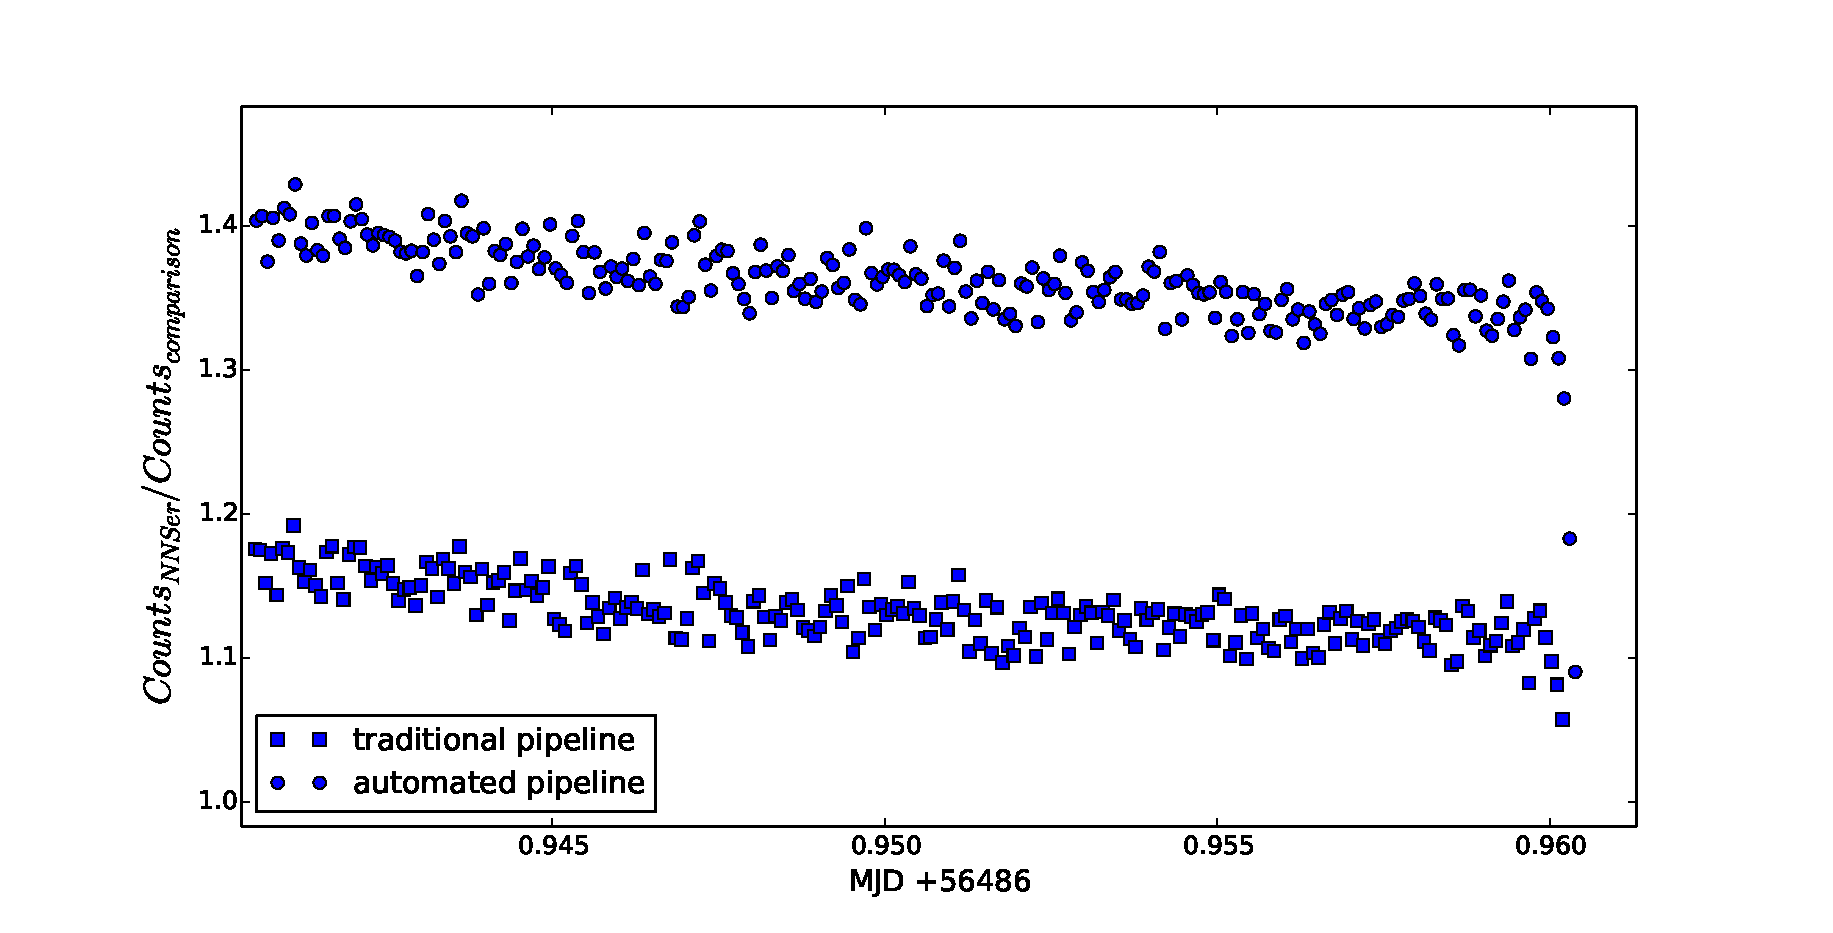
\includegraphics[width=140mm]{images/nn_ser_compare_zoom_b.eps}
\caption{A closer look at the comparison of the light-curves for NN Ser in the Sloan u filter, from the start of the run to the beginning of the eclipse ingress. Square data points were generated by the traditional pipeline and circles by the automated pipeline. The vertical offset applied to the circles is 0.23. }
\label{fig:comparepipelines_zoom_b}
\end{figure}

Since the automated pipeline relies on the third party software, SExtractor, to determine the apertures on each frame, objects that do not meet the required signal-to-noise ratio on any particular frame will not be detected and therefore have no aperture defined for that frame. No aperture means that we will have no photometry. This has the result that objects that fade or are generally quite faint might disappear on some frames and then re-appear on subsequent frames. The tracking algorithm allows a re-appearing object to be identified with an object that had previously disappeared on earlier frames provided that the pixel location is roughly similar. An illustration of this can be seen in figures \ref{fig:comparepipelines_g} and \ref{fig:comparepipelines_b} where the automated pipeline loses the target in the `g' and `u' bands after the ingress of the primary eclipse, but picks it up again at the start of egress. In contrast, the traditional pipeline can have apertures that are linked to other objects in the field and can therefore continue to measure flux in the aperture for the target even if the target is not detectable above the sky background.

% \begin{figure}
% \centering
% 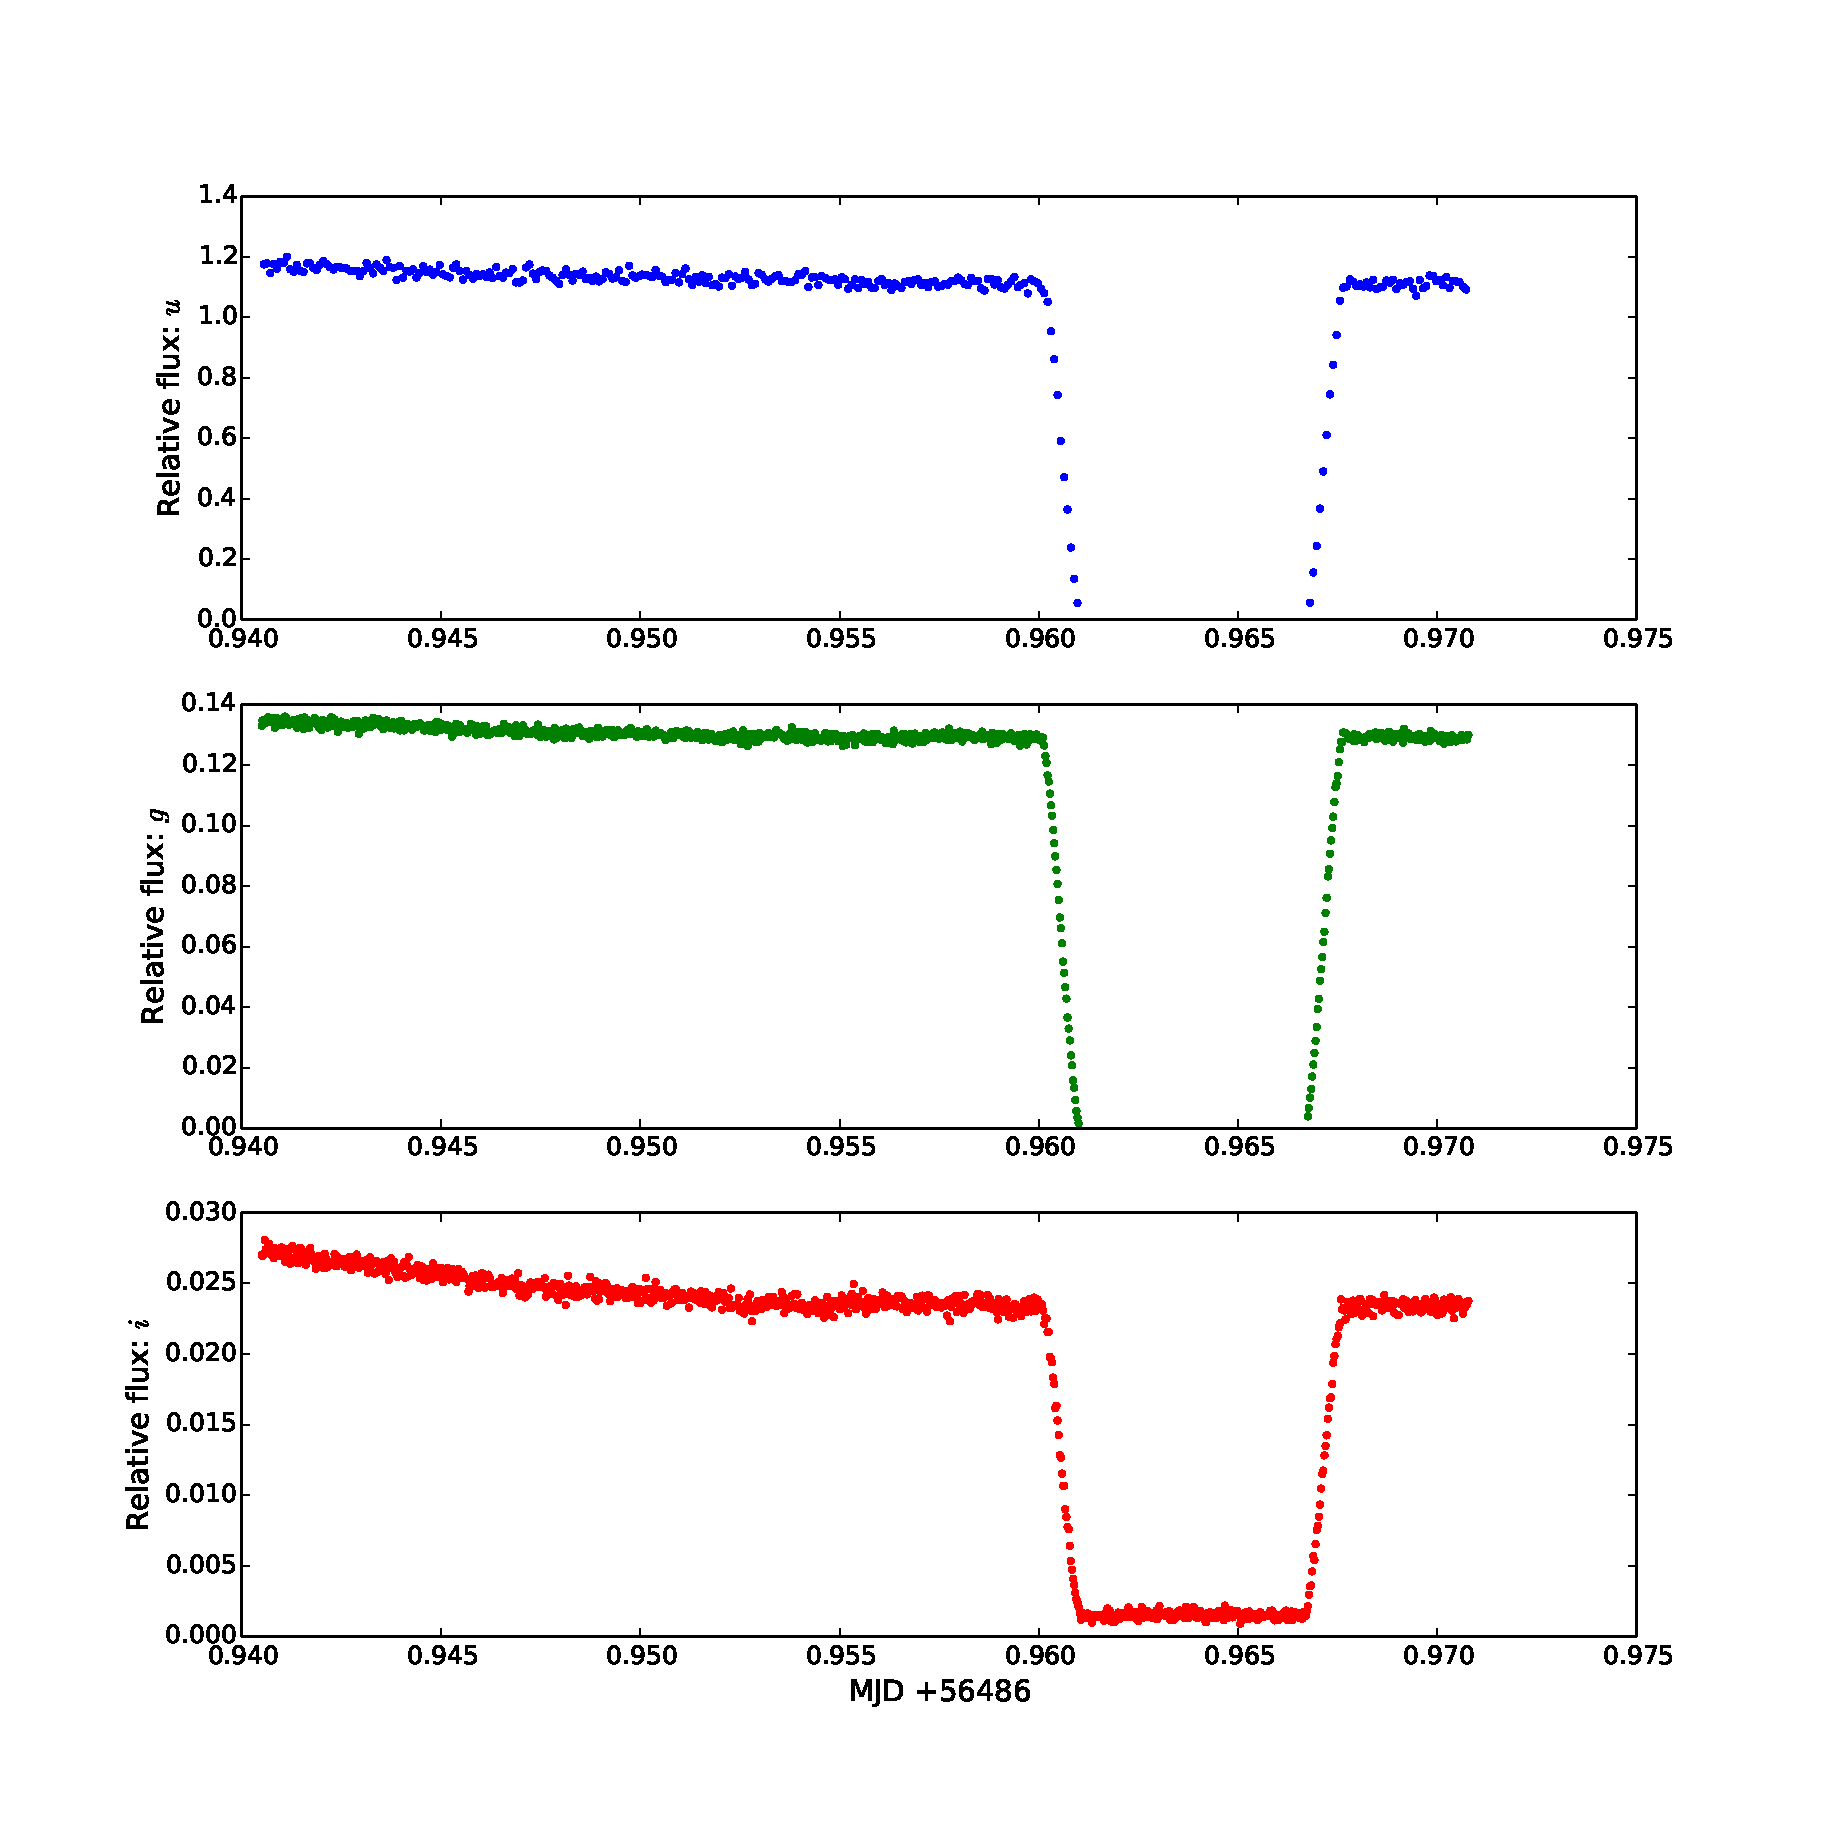
\includegraphics[width=140mm]{images/nnser_lightcurve_automated.eps}
% % % % \caption{Light curve of the target object, NN Ser produced using the \emph{automated pipeline}. The intensity of the target is plotted as its flux relative to the comparison star in the field. The red, green and blue data points are the measurements taken in the Sloan i, g, and u filters, respectively. Note that the automated pipeline (previous figure) completely loses the target in the $u$ and $g$ filters during the primary eclipse. In contrast, the traditional pipeline maintains readings of the target throughout the eclipse. This is due to the fact that the automated pipeline creates new apertures for each frame and the target is too faint during the eclipse to trigger the aperture creation for this object.}
% \label{fig:nnserlightcurveautomated}
% \end{figure}

% \begin{figure}
% \centering
% 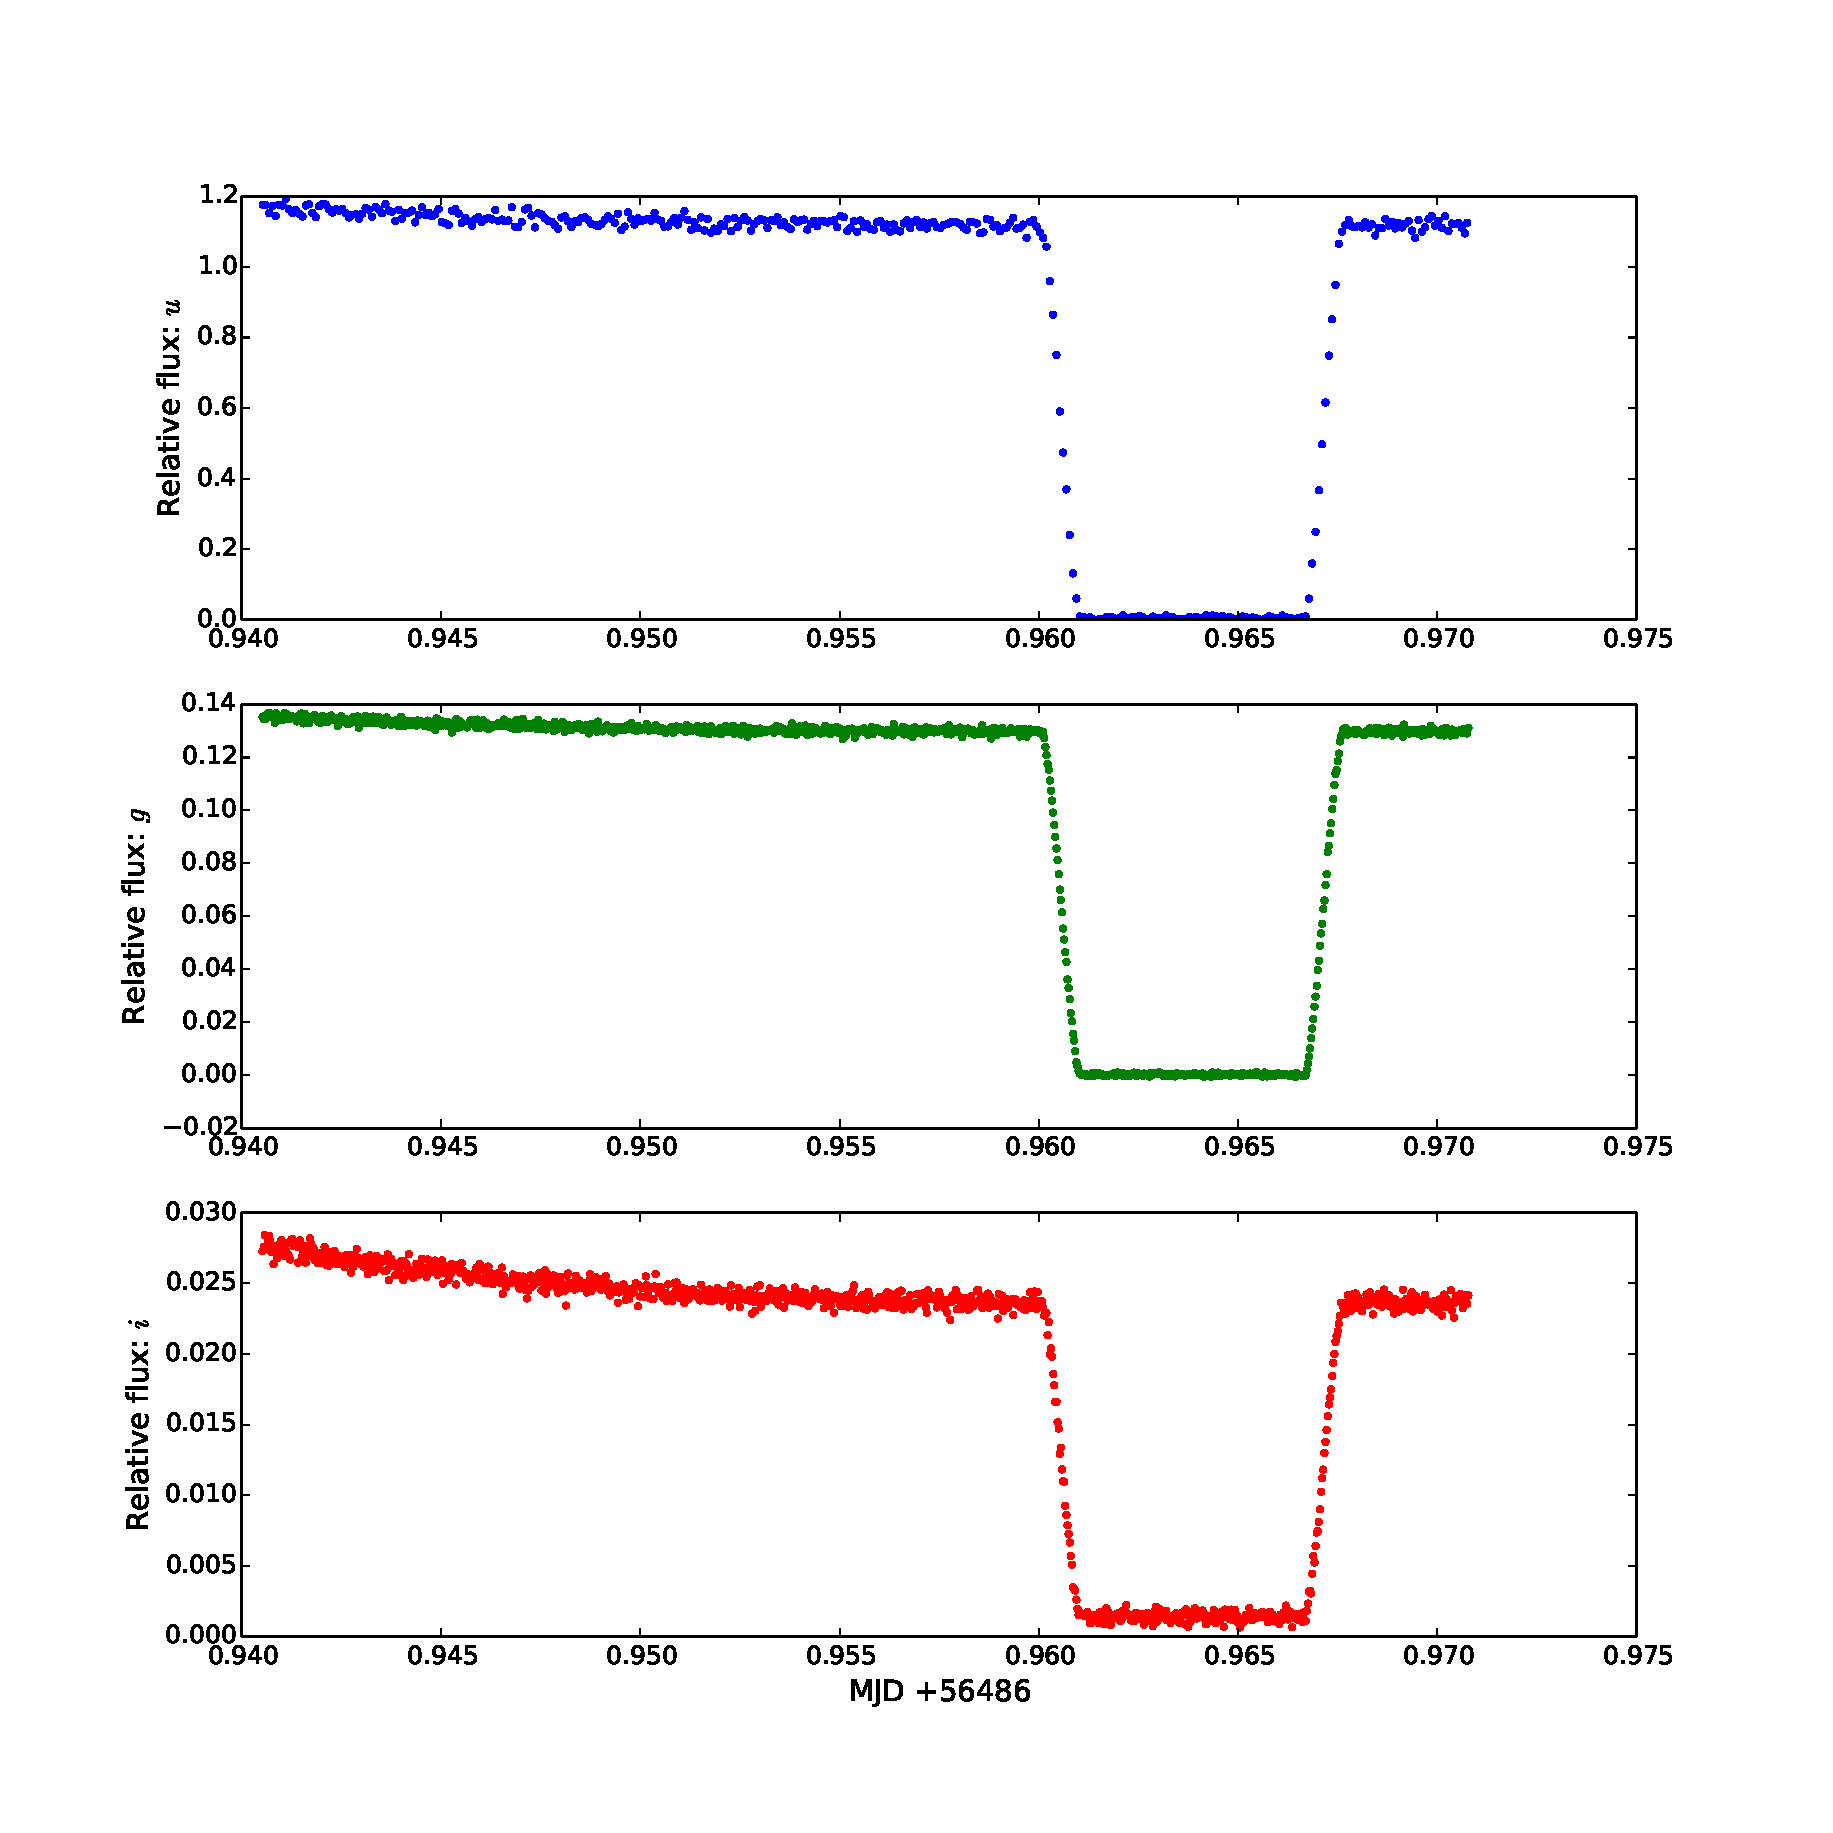
\includegraphics[width=140mm]{images/nnser_lightcurve_tom.eps}
% \caption{Light curve of the target object, NN Ser, produced using the \emph{standard pipeline}. The intensity of the target is plotted as its flux relative to the comparison star in the field. The red, green and blue data points are the measurements taken in the Sloan i, g, and u filters, respectively. }
% \label{fig:nnserlightcurvetom}
% \end{figure}

As an alternative to comparing the light-curves side-by-side a check the systematic differences between the pipelines can be performed by comparing their measured flux values for a particular object to each other. Both pipelines were used to produce light-curves for the comparison star labeled `0' in figure \ref{fig:nnserfield}. Rather than plotting each light-curve separately, they are plotted as the counts measured by the automated pipeline divided by the counts measured by the traditional pipeline. This is shown in figure \ref{fig:comparephotometry}. The task was then repeated for object `3' and is shown in figure \ref{fig:comparephotometry2} The statistics of this data set are shown in table \ref{tab:differential}. The traditional pipeline gives a slightly higher reading for the overall flux than the new automated pipeline, resulting in a mean that is less than unity. The likely cause of this is the different size of aperture used by each pipeline. This will be investigated as the pipeline is enhanced to give calibrated photometry in future versions. 

As a deeper examination of the systematics between the two pipelines, the relative flux counts measured in each pipeline were plotted as a ratio of each other. First, the relative flux of object `3' to object '0' in the automated pipeline, $F_{auto}$ was calculated and then the same relative flux for the same two objects as measured by the traditional pipeline, $F_{trad}$. The plot shown in figure  \ref{fig:difference-of-ratios} was produced by computing the ratio of these two data sets and subtracting 1,  $\frac{F_{auto}}{F_{trad}} - 1$. The amplitude of the scatter is on the order of 1\% in the blue channel and 0.1\% for the red and green channels. 

\begin{figure}
\centering
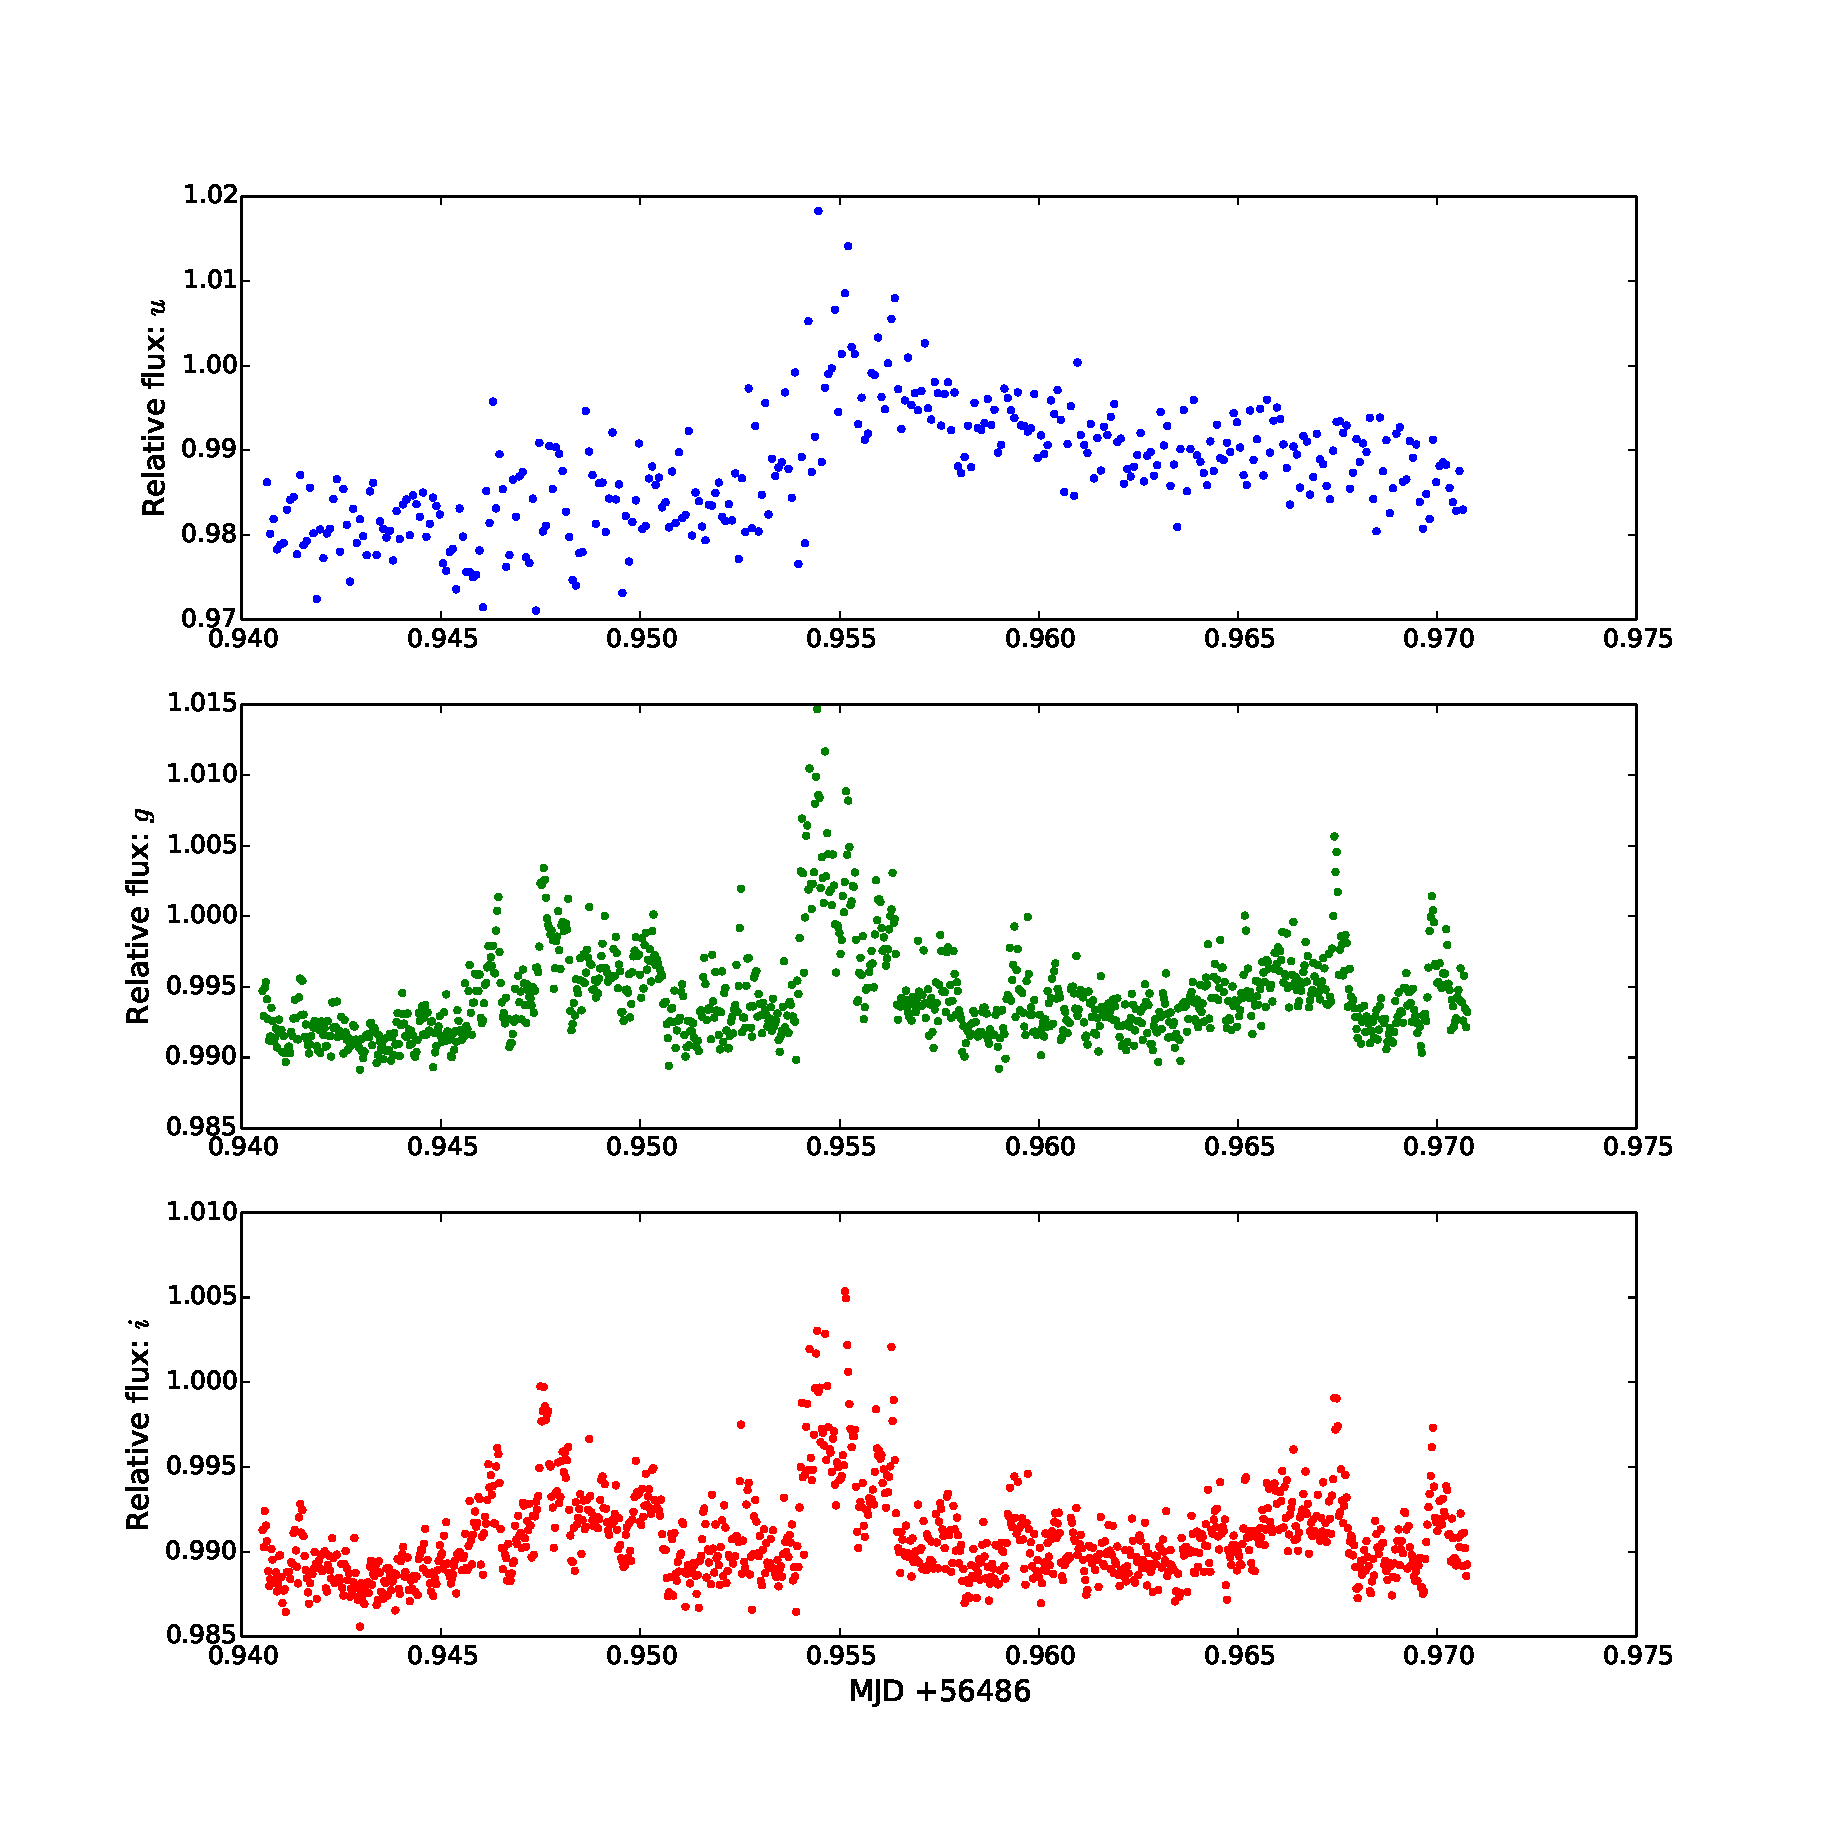
\includegraphics[width=140mm]{images/compare_photometry.eps}
\caption{Object 0: A comparison of the flux measurements for a single object labeled `0' in figure \ref{fig:nnserfield}. The plot is produced by dividing the flux counts as measured by the \emph{automated} pipeline by the flux counts as measured by the \emph{traditional} pipeline.}
\label{fig:comparephotometry}
\end{figure}

\begin{figure}
\centering
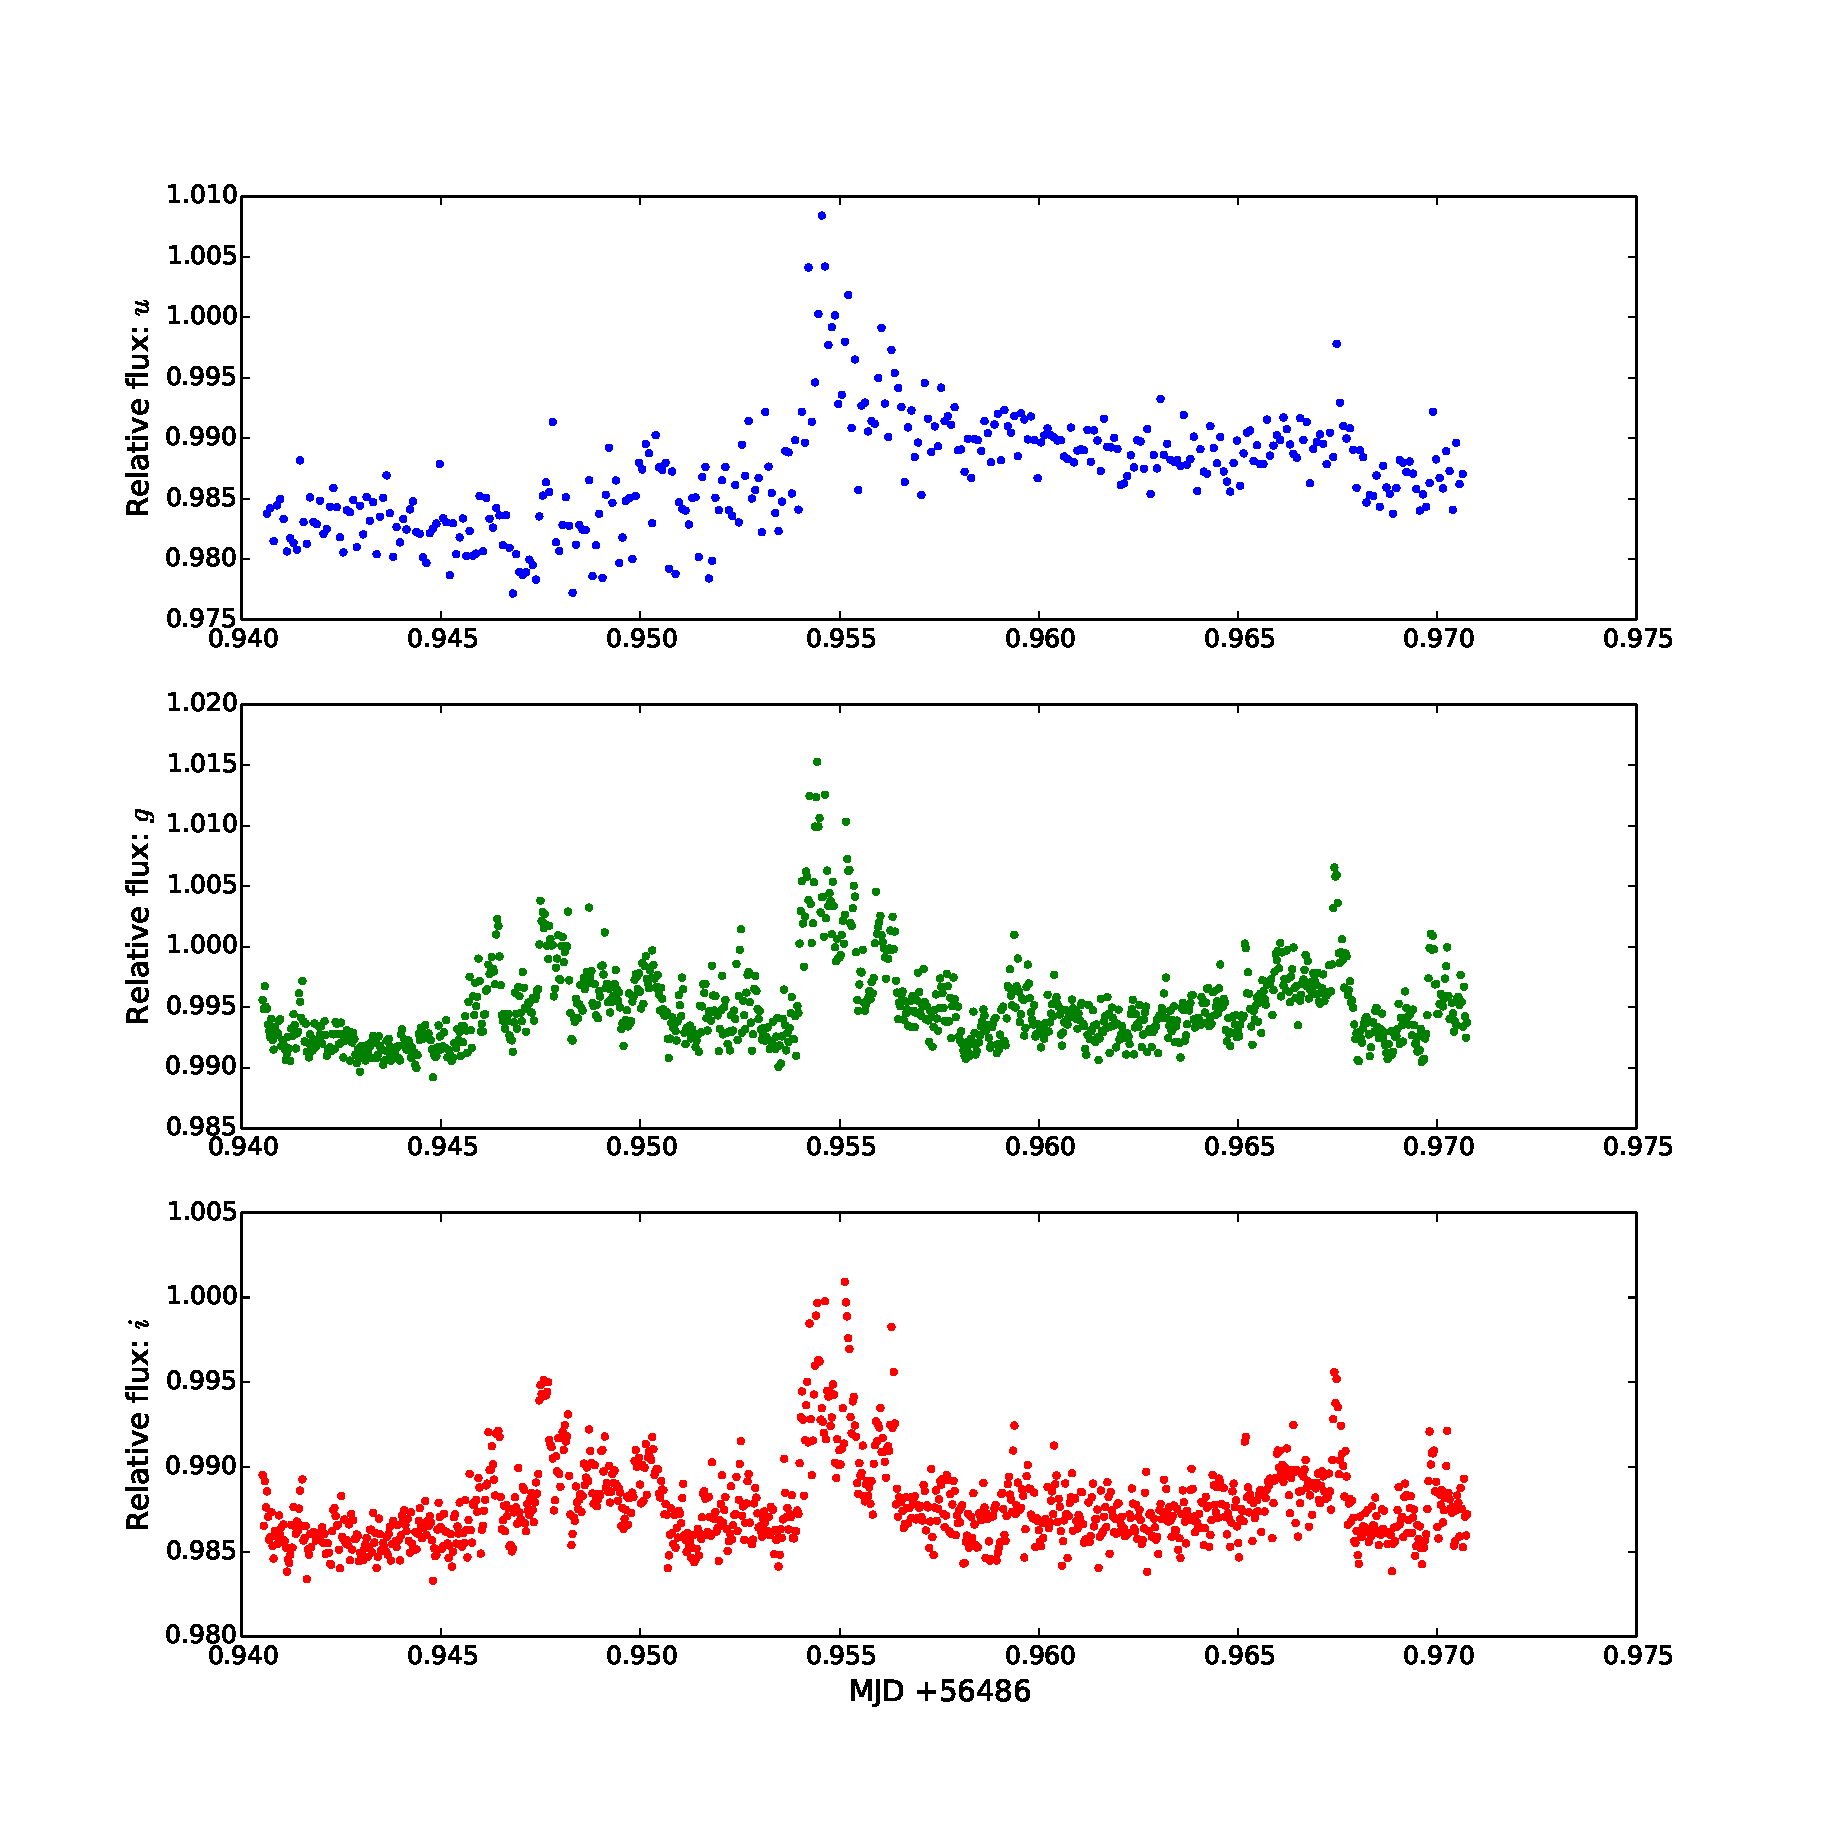
\includegraphics[width=140mm]{images/compare_photometry_2.eps}
\caption{Object 3: A comparison of the flux measurements for a single object, labeled `3' in figure \ref{fig:nnserfield}. The plot is produced by dividing the flux counts as measured by the \emph{automated} pipeline by the flux counts as measured by the \emph{traditional} pipeline. Comparing this plot to the similar plot for object `0' in figure \ref{fig:comparephotometry} shows very similar systematics.}
\label{fig:comparephotometry2}
\end{figure}

\begin{table}
  \centering
  \begin{tabular}{l r r }
    \hline
    Filter & Flux ratio for object `0' & Flux ratio  for object `3'\\
           &  $mean[std. dev]$ &  $mean[std. dev]$\\
    \hline
    `i'    & 0.991[0.003]  & 0.989[0.003] \\
    `g'    & 0.994[0.003] & 0.991[0.003]\\
    `u'    & 0.988[0.007] & 0.987[0.007]\\
    \hline
   \end{tabular}
  \caption{Table showing the statistics of the photometry produced by dividing the flux counts from the automated pipeline by the flux counts from the traditional pipeline for objects `0'  and `3' in figure \ref{fig:nnserfield}.}
  \label{tab:differential}
\end{table}

\begin{figure}
\centering
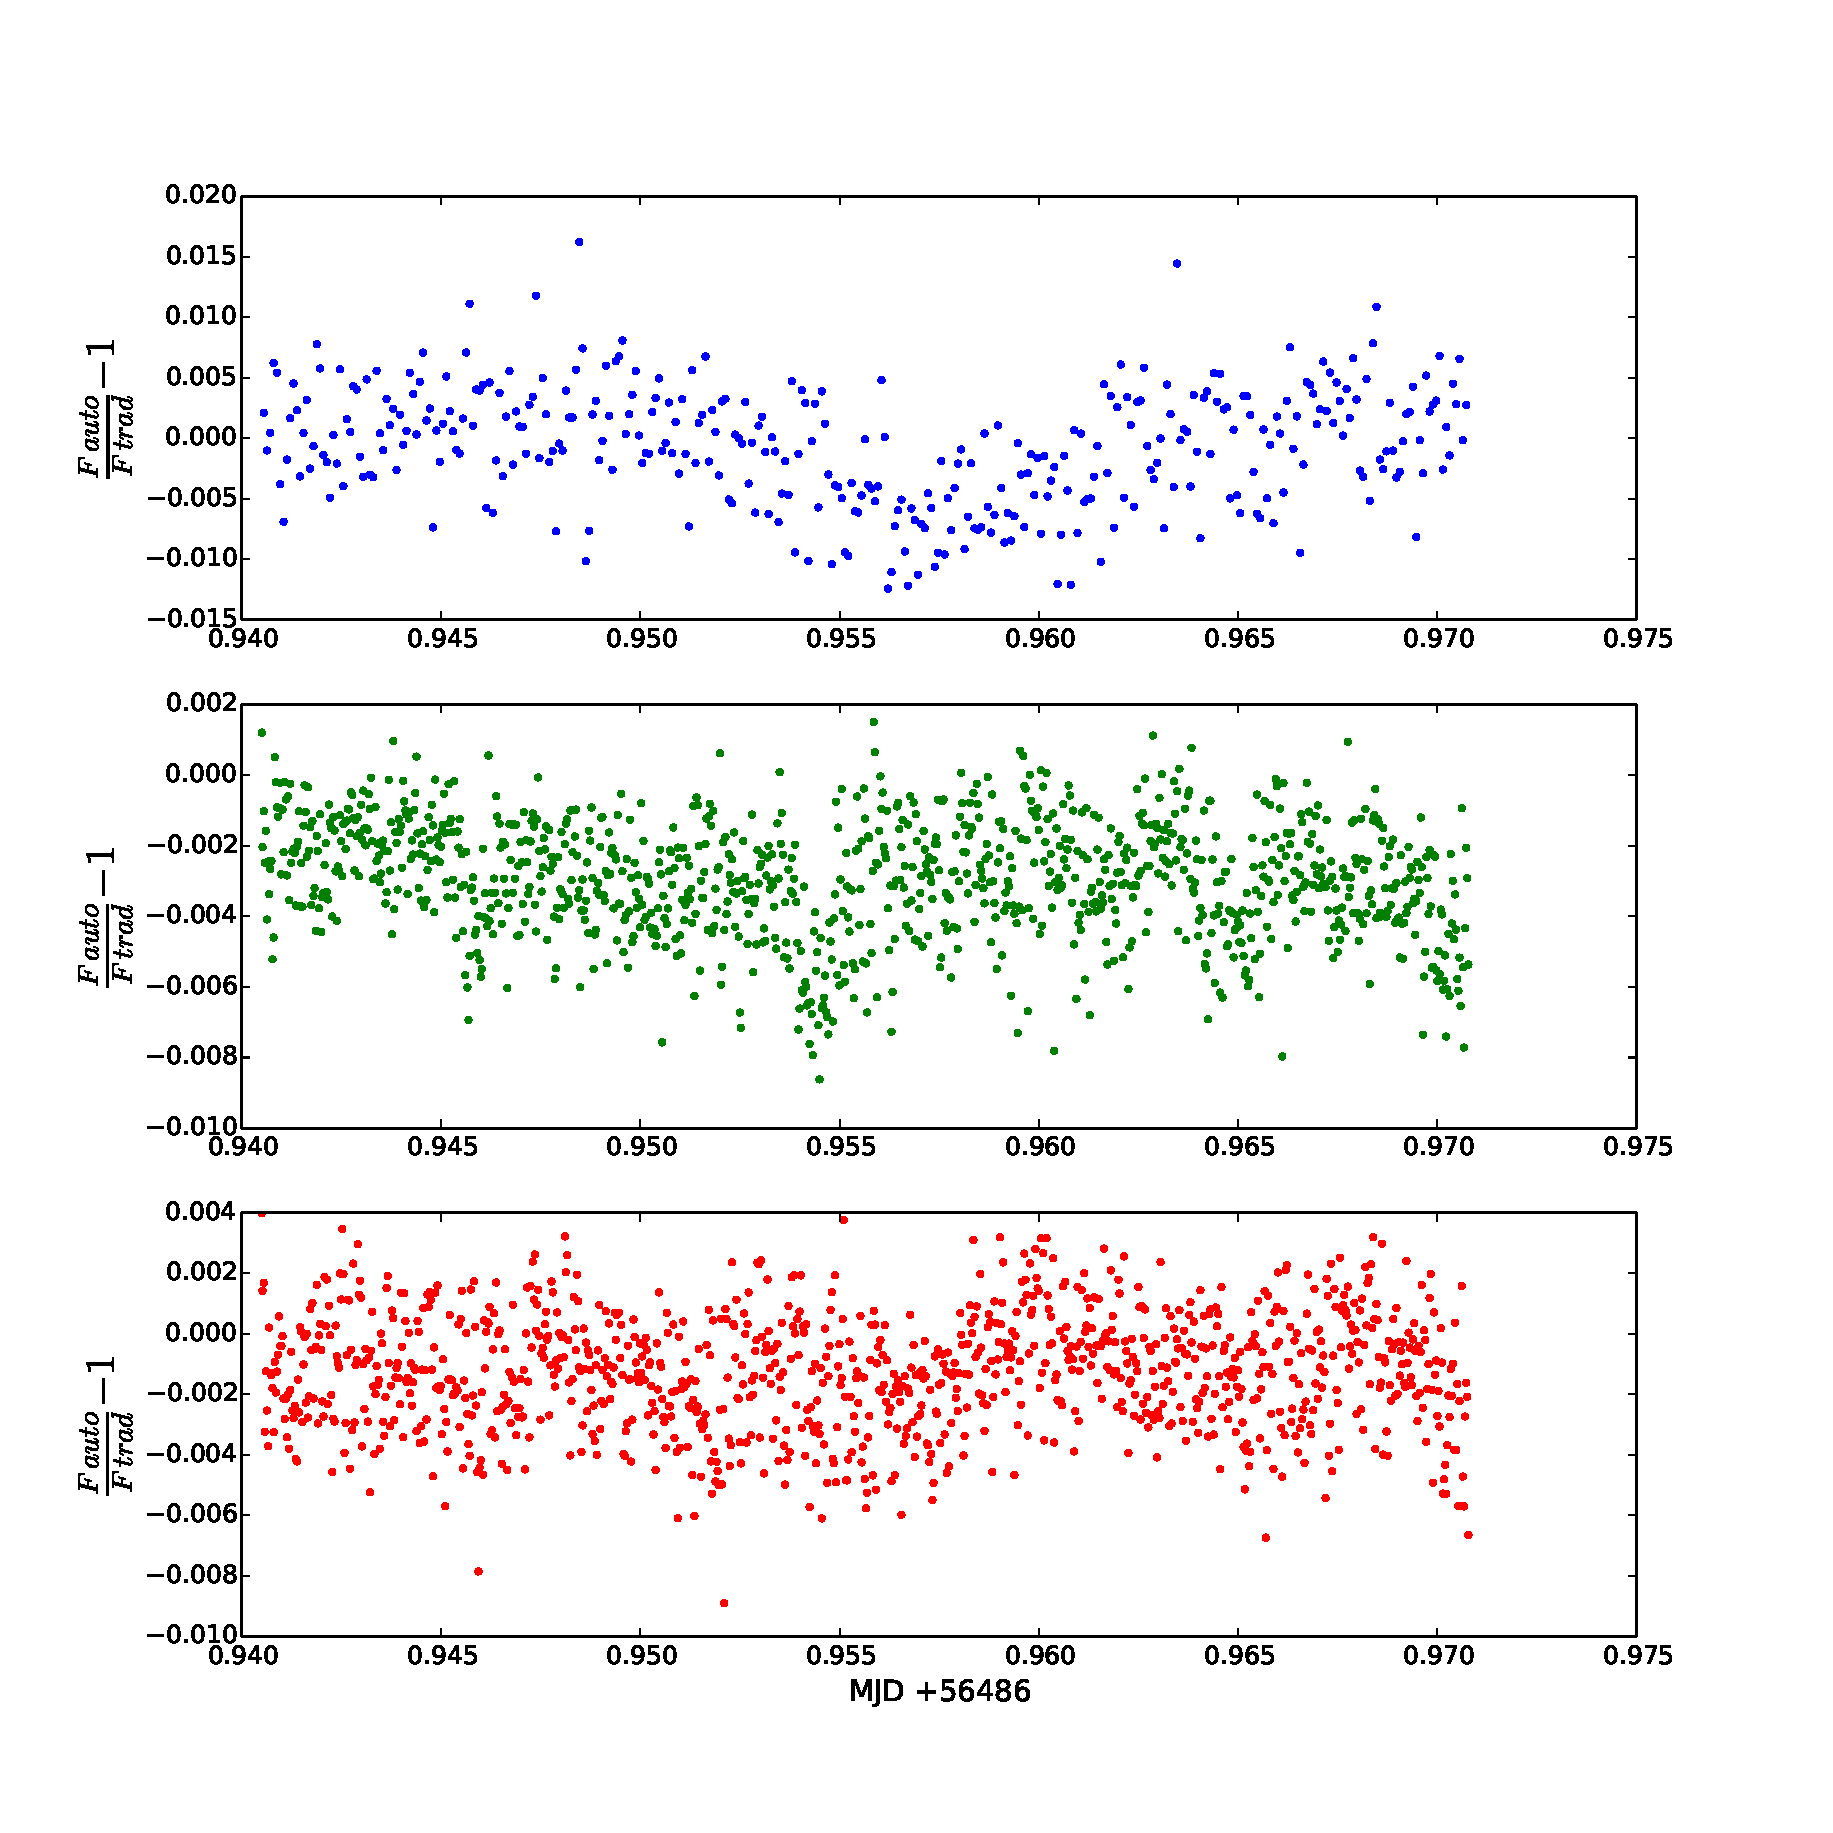
\includegraphics[width=140mm]{images/ratio-of-ratios.eps}
\caption{Traditional pipeline vs the automated pipeline: A comparison of the flux ratios, defined as $\frac{F_{auto}}{F_{trad}} - 1$ , where $F$ is the relative flux counts for object `3' to object `0' as measured by each pipeline, automated and traditional.}
\label{fig:ratio-of-ratios}
\end{figure}


\section{Object matching accuracy}
As discussed in chapter \ref{chap:datareduction}, the automated pipeline can struggle to cross-identify the same object across in the three channels, r, g, b. This is usually only a problem in crowded fields where the average pixel position of the object does not clearly distinguish it from nearby objects. In other words, an object might have been identified as the same object in the blue channel (due to its proximity on the image) but is actually a merely a neighbour to this object in the red and green channels, so the pipeline has mistakenly assigned all three measurements as belonging to the same object.

By plotting colour-colour and colour-magnitude diagrams for a few of the crowded fields in the ULTRACAM archive we can get an indication of the severity of this mis-matching problem. Although the automated pipeline does not perform a calibration of the magnitudes of the objects it is still possible to create colour-colour diagrams provided that we are not concerned with the correct offsets for our $(u-g)$ and $(g-r)$ axes. We can also produce a colour-magnitude diagram if we have a field that contains objects that are all at the same distance from us. In these automatically-produced plots, there are some outliers showing colours that are too extreme to be genuine astronomical bodies. 

\begin{figure}
\centering
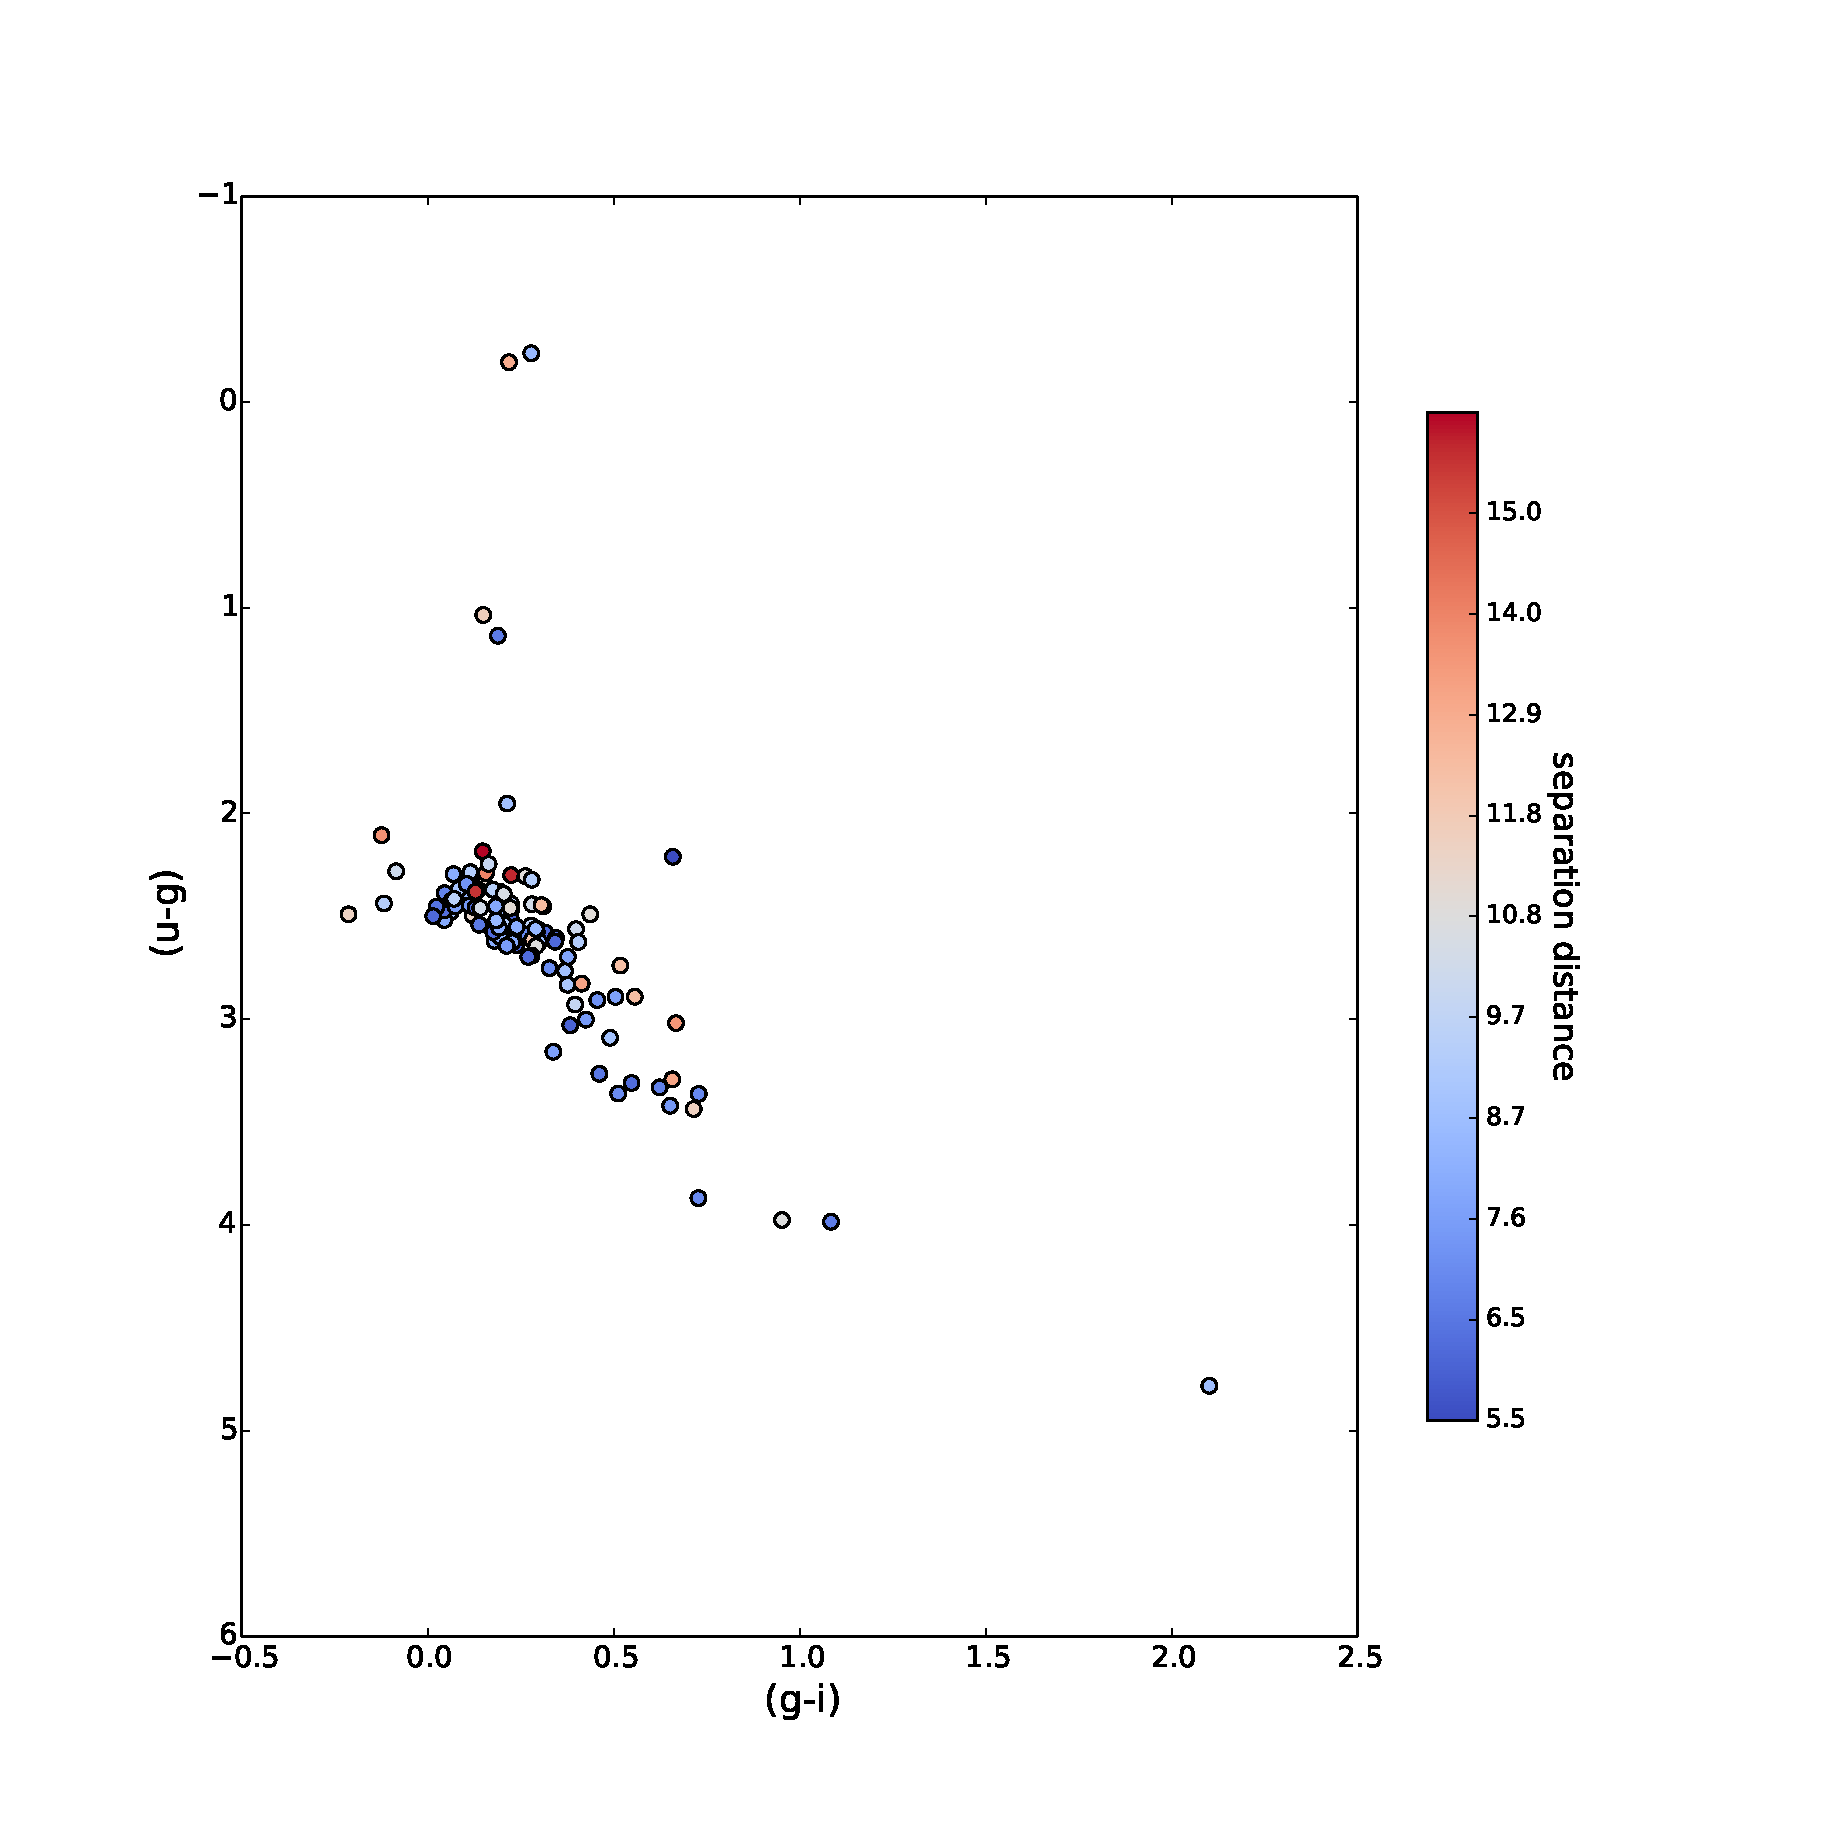
\includegraphics[width=140mm]{images/2013-07-21-run010-2colour.eps}
\caption{The colour-colour plot of run: \emph{2013-07-21/run010}. The plot contains 110 objects located near the Kepler exoplanet host KIC5115978. The offsets on the x and y axes are both arbitrary as the photometry has not been calibrated with photometric standards. The outliers with extreme red and blue colours are due to mistaken classification by the automated pipeline. The colour map indicates how separated the $(x, y)$ positions for the object are in each of the 3 channels.}
\label{fig:run010-2colour}
\end{figure}

\begin{figure}
\centering
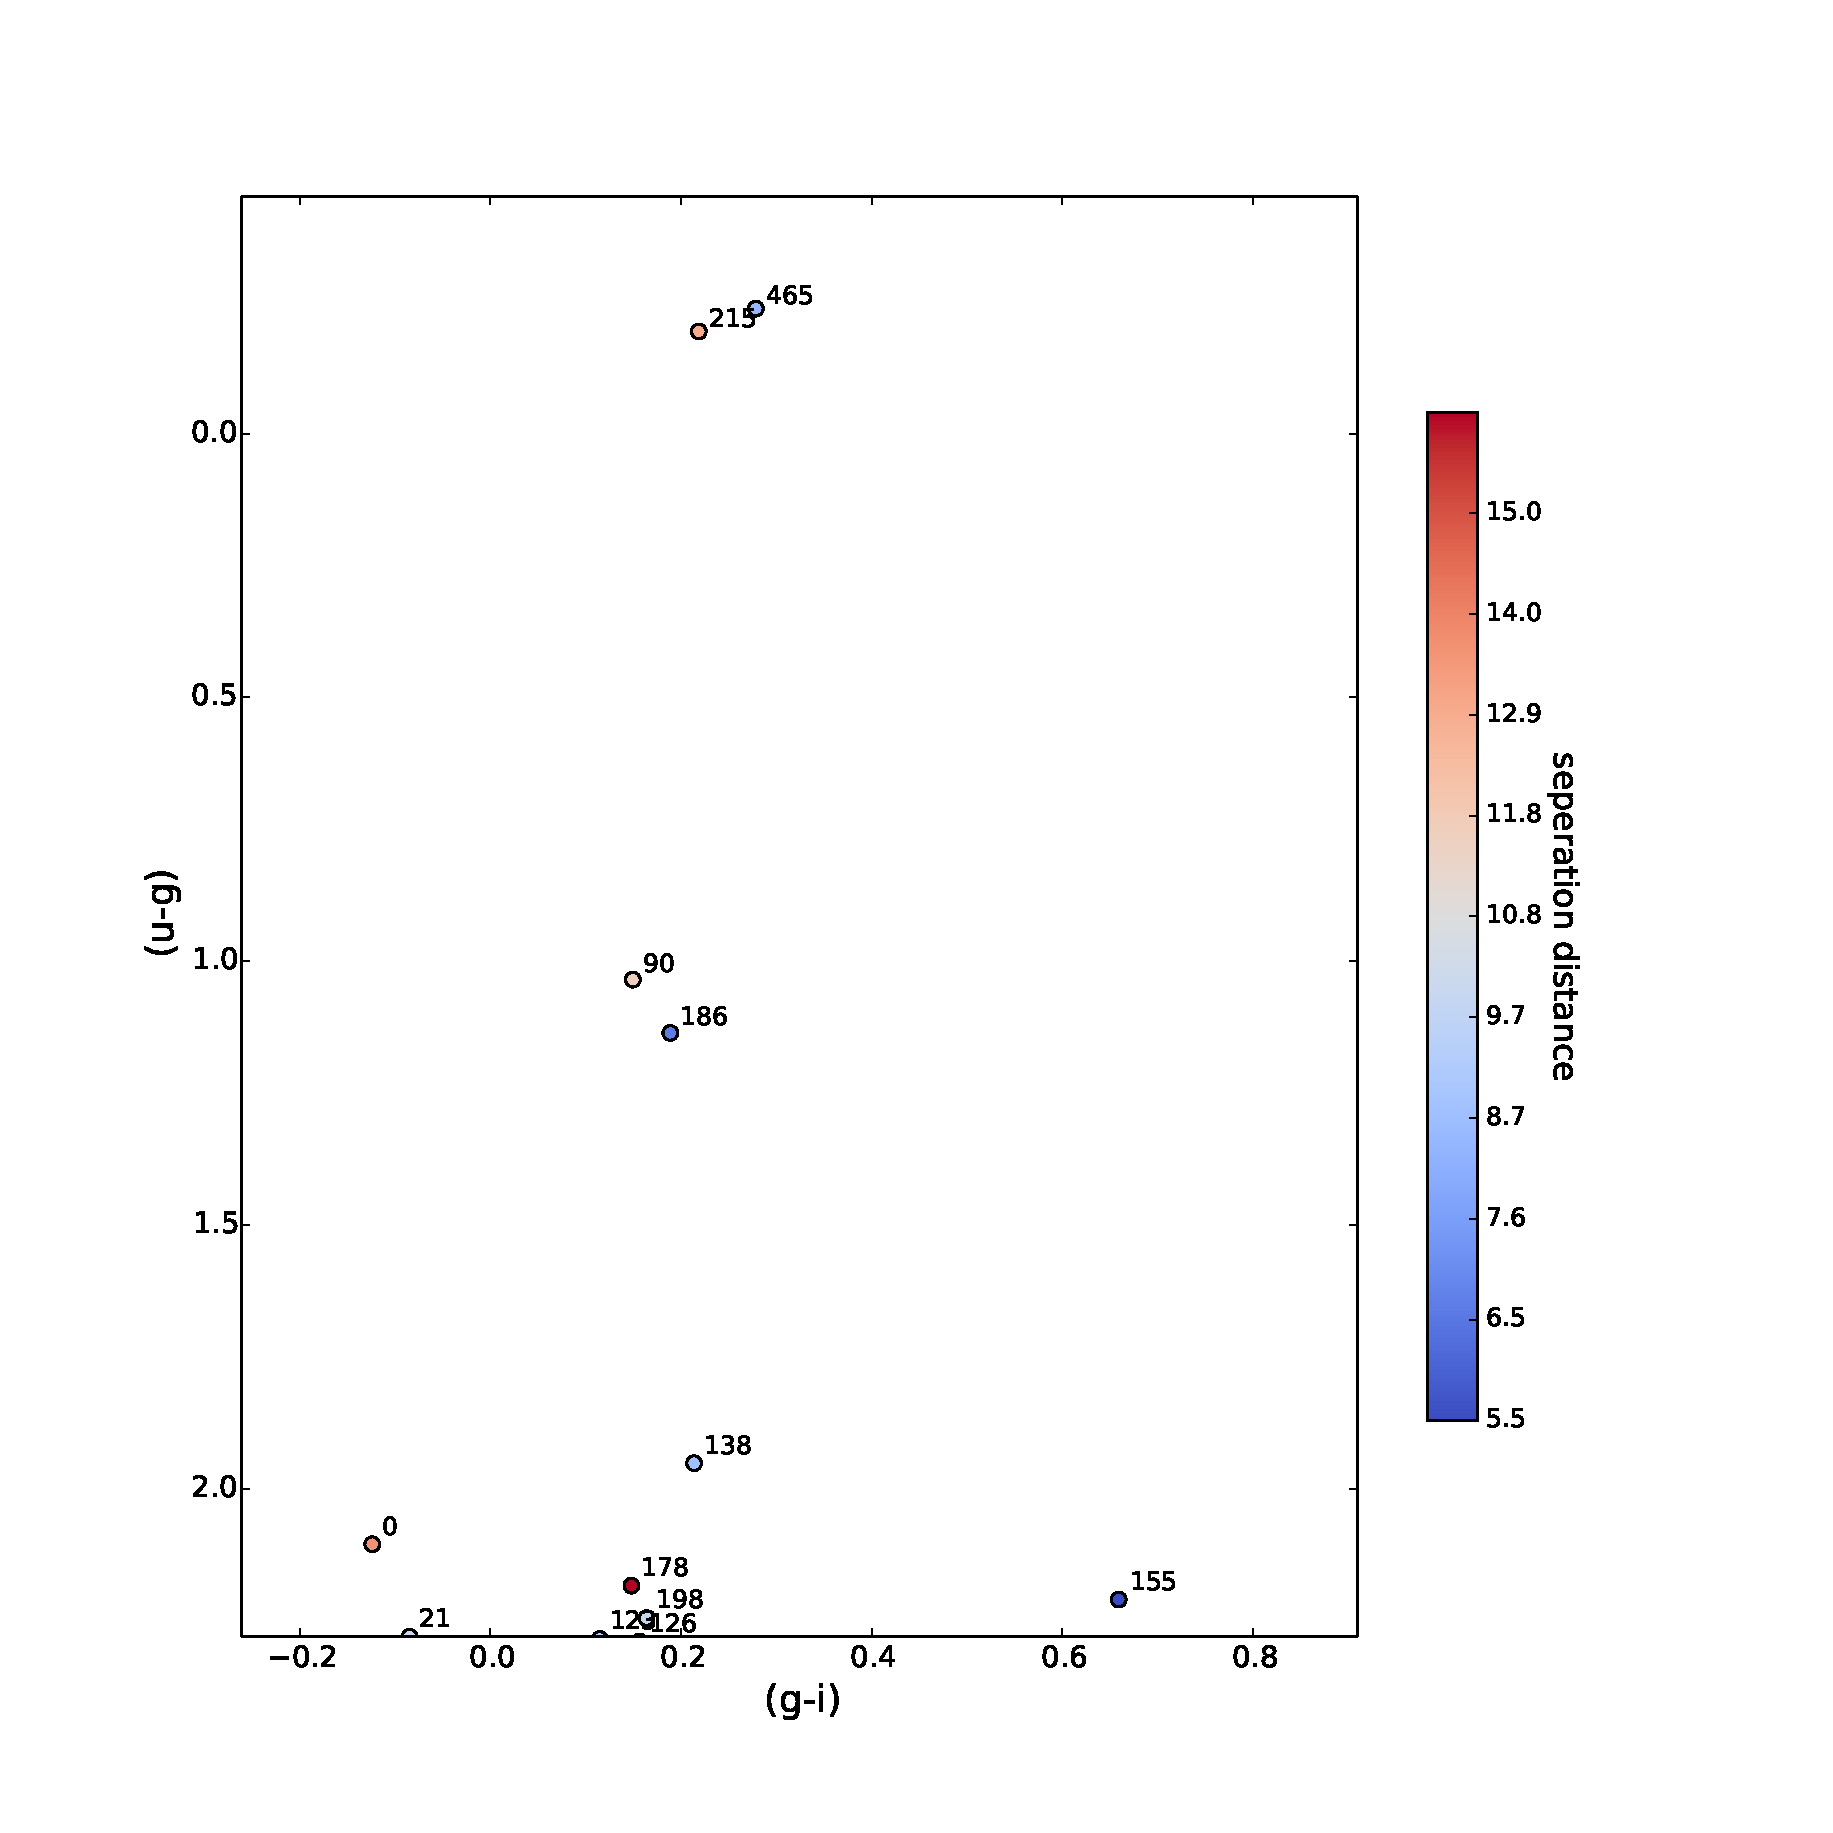
\includegraphics[width=120mm]{images/colour-colour-zoom-with-labels.eps}
\caption{A closer look at some of the outliers in figure \ref{fig:run010-2colour} showing the automated pipeline's identification label for each object. Going back to the web browser and inspecting them shows that both of the object's labeled `465' and `215' were mis-identified in the blue channel. }
\label{fig:run010-2colour-zoom}
\end{figure}

\begin{figure}
  \centering
  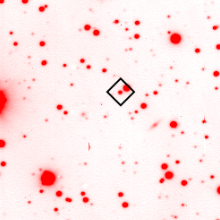
\includegraphics[width=.30\linewidth]{images/mismatch-run010_r.png}
  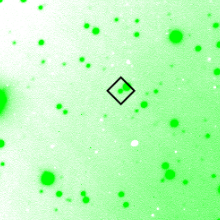
\includegraphics[width=.30\linewidth]{images/mismatch-run010_g.png}
  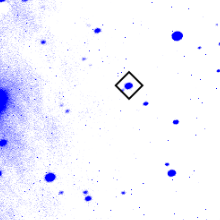
\includegraphics[width=.30\linewidth]{images/mismatch-run010_b.png}
  \caption{Checking the matching of the colour-colour outlier labeled `465' in figure \ref{fig:run010-2colour-zoom}. The object has been incorrectly identified with a neighbour that is brighter in the blue channel.}
\label{fig:comparewebmismatch}
\end{figure}

In figure \ref{fig:run010-2colour} we have plotted a colour-colour diagram of run \emph{2013-07-21/run010}. In this diagram it is clear that there are some outliers. If we zoom in (see figure \ref{fig:run010-2colour-zoom}) and show the labels the objects as they have been identified in the automated pipeline, we can go back to the web interface to check if the cross-identification has worked correctly. An outlier in figure \ref{fig:run010-2colour-zoom} is identified as object `465' in the run. Looking at figure \ref{fig:comparewebmismatch} we can see that the pipeline has incorrectly identified a neighbour of this object in the blue channel as it was brighter in blue and relatively nearby. Figure \ref{fig:run010-2colour} uses a colour map to show the relative distances of the object from channel to channel. The relative distance has been calculated by taking the Pythagorean distance ($D$) of the object's separation from the red to the green channel, ($D_{rg}$) and the object's separation from the red to the blue channel, ($D_{rb}$).  \begin{equation}D = \sqrt{ D_{rg}^2 + D_{rb}^2}\end{equation}where \begin{equation}D_{rg} = \sqrt{ (x_r - x_g)^2 + (y_r - y_g)^2}\end{equation} and \begin{equation}D_{rb} = \sqrt{ (x_r - x_b)^2 + (y_r - y_b)^2} \end{equation}.

It seems that this separation distance $D$ is not clear discriminator of whether an object is matched correctly. In crowded fields, confusion occurs when objects are close together. Setting the minimum matching distance threshold to a lower value does not significantly reduce the number of mismatches. In fact, the systematic differences between each of the channels are larger than the separation of individual objects on each field. An effect that becomes more pronounced when objects are near to the edges of the CCD. This can also be seen in figures  \ref{fig:nonoverlap}, \ref{fig:greentored} and \ref{fig:bluetored}.  We conclude that in order to address this issue with the pipeline we need a more robust algorithm for clearly identifying each object's position in each of the channels (perhaps with an accurate WCS solution) and then performing the cross identification. 

\begin{figure}
\centering
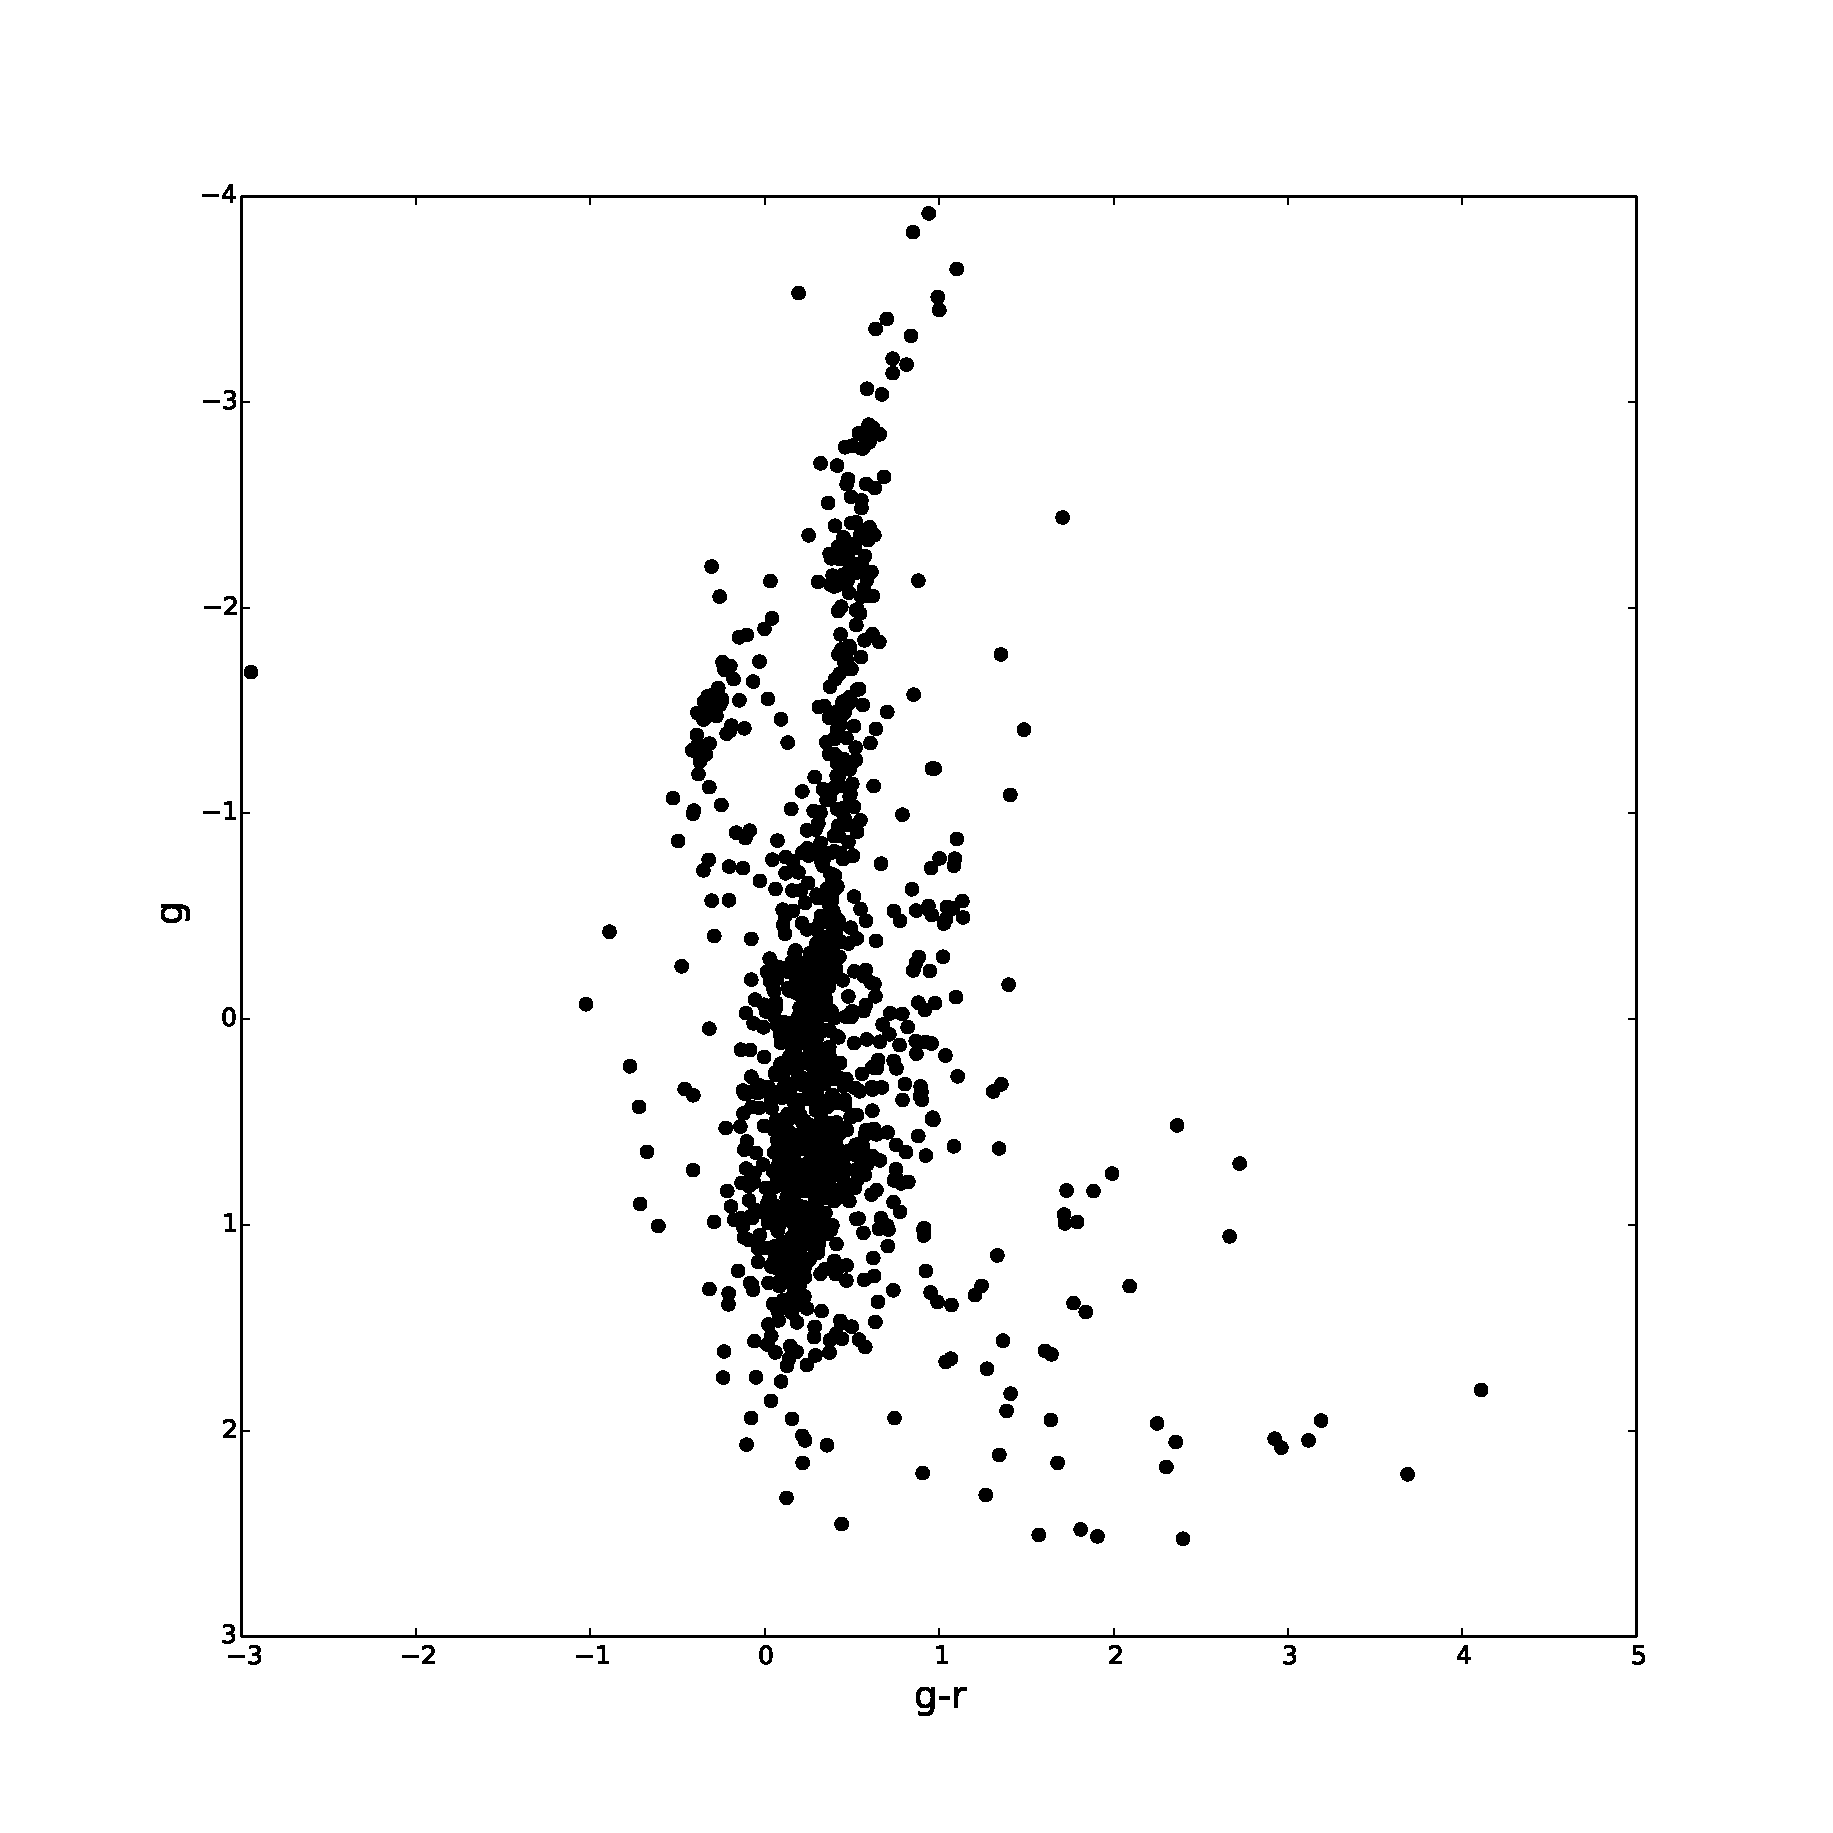
\includegraphics[width=120mm]{images/2011-04-22-run019-omegacen-colourmagnitude.eps}
\caption{A colour-magnitude plot of run: \emph{2011-04-22/run019}. The plot includes 1087 objects found in a field taken of the outer perimeter of the globular cluster \emph{Omega Centaurus}. The offsets on the x and y axes are both arbitrary as the photometry has not been calibrated to photometric standards. }
\label{fig:OmegaCen-colourmagnitude}
\end{figure}

The ULTRACAM archive includes a run covering the outskirts of the globular cluster, Omega Centaurus, recorded at the NTT on the night of 2011-04-22.  Since all of the objects are at a similar distance to us, assuming no foreground or background contamination, we can use this run to produce a colour-magnitude diagram of the cluster. This is shown in  figure \ref{fig:OmegaCen-colourmagnitude}. 

% \begin{figure}
% \centering
% 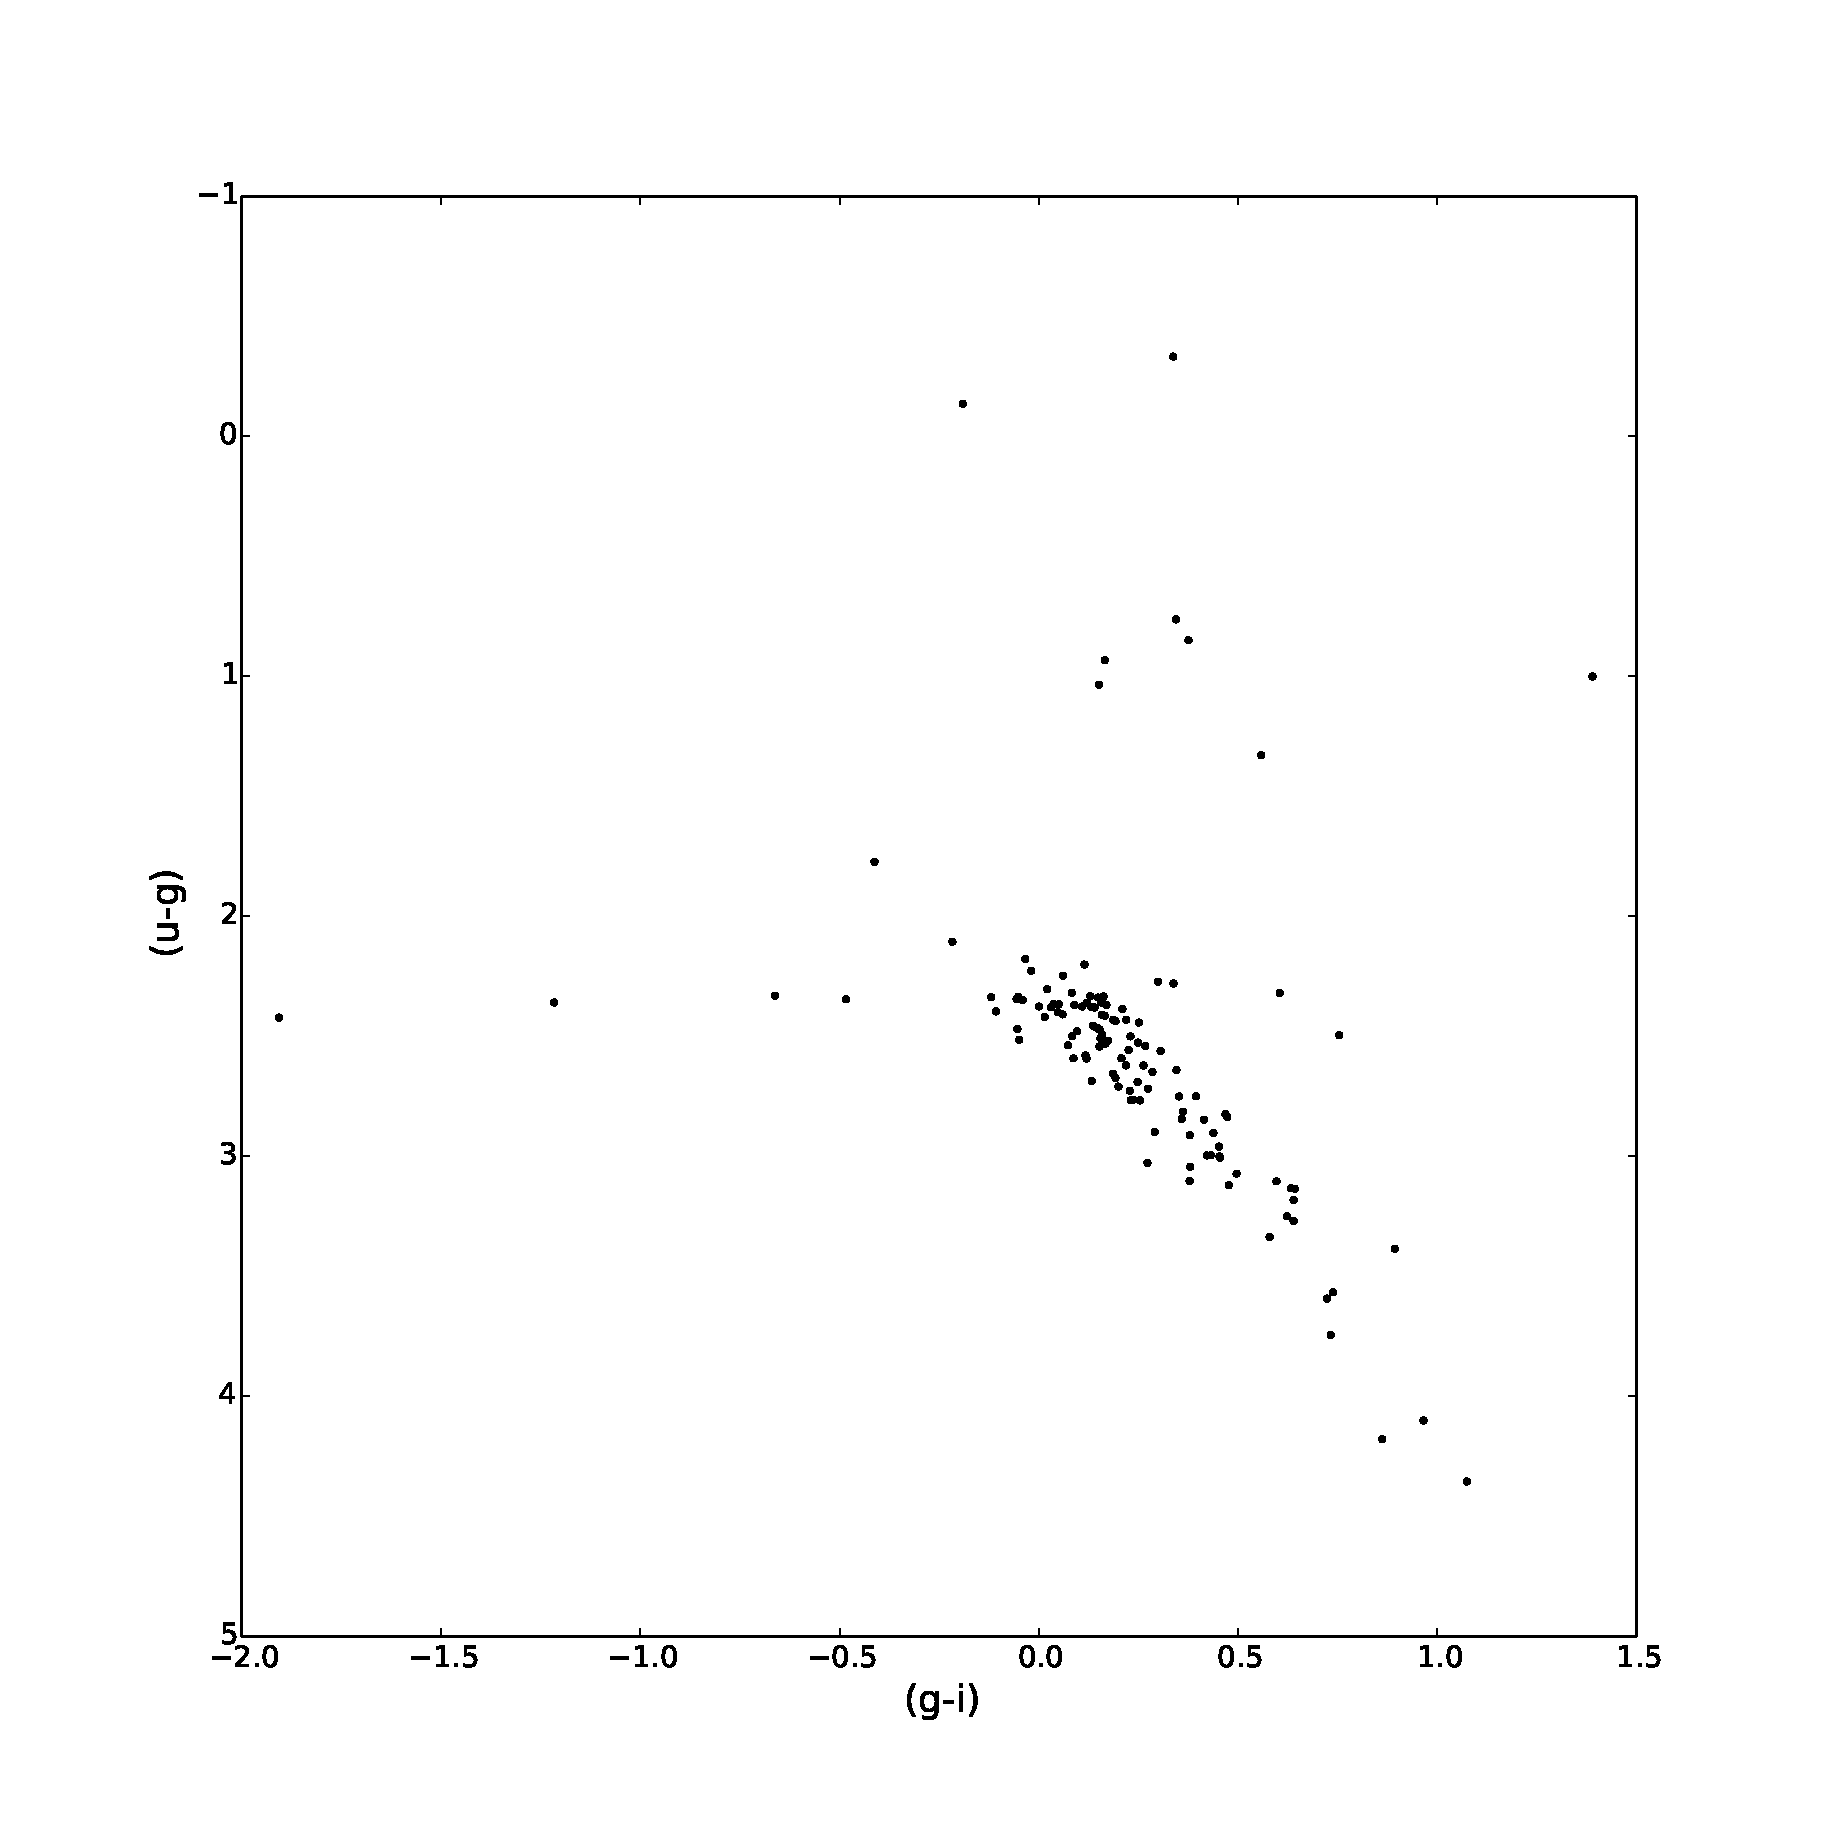
\includegraphics[width=120mm]{images/2013-07-21-run011-2colour.eps}
% \caption{The colour-colour plot of run: \emph{2013-07-21/run011}. The offsets on the x and y axes are both arbitrary as the photometry has not been calibrated with photometric standards. The outliers with extreme red and blue colours are due to mistaken classification by the automated pipeline. }
% \label{fig:run011-2colour}
% \end{figure}


\section{Finding variable objects}
In this section we present three examples of how the web interface makes browsing the ULTRACAM archive quick and easy and thereby enables the discovery of new variable objects. These objects were found in July 2014 when Matthew Green, who was a summer student at the University of Warwick and I were looking through web pages produced by the new pipeline.

\subsection{X-ray transient: GU Mus}
The first example is the serendipitous discovery of {GU Mus}, the X-ray transient object that was observed in quiescence in May 2005 at the VLT. We originally suspected that it was a cataclysmic variable. {GU Mus} was at magnitude of 20.65 in Sloan g at the time, \citep{tariq2010}. Because it was fairly faint, we assumed it was not the intended target. Since ULTRACAM data does not include the pixel position of the target object in the field, it was not obvious which one out of the 205 objects identified by the pipeline was {GU Mus}. The normal method for finding the target object is to revert to finding charts and existing catalogs. Figure \ref{fig:gumus-discovery} contains image captures from the web browser interface showing how the light-curves and the field are presented to the user. By pressing the `left' and `right' arrow keys, the user can scroll through all of the light-curves like pages in a book. For this run, there were 205 individual light-curves available for browsing but by quickly flipping through them the user can spot any obvious variability. Most objects show light-curves similar to the upper one in figure \ref{fig:gumus-discovery} with no obvious variability above the noise. The object with the identification number `58' however, was showing clear evidence of flickering. We assumed that we had discovered a new CV. Since {GU Mus} is a faint object, it took us a day to find an accurate finding chart. When we did so, we realised that our `new' variable was actually {GU Mus} itself. Although our initial excitement was dampened, this incident can be seen as good evidence that the automated pipeline and the browser interface is capable of revealing faint variable objects. As a bonus, the object just a few arc minutes to the right turned out to be variable too. It is a {W UMa} variable and is discussed in chapter \ref{chap:highlights}.

\begin{figure}
\centering
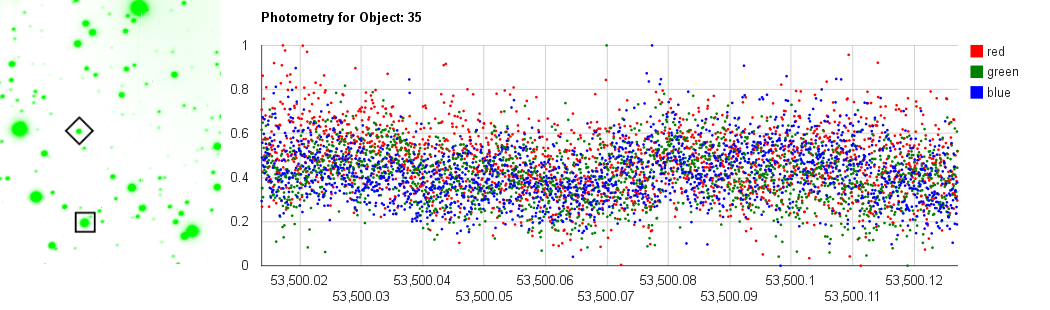
\includegraphics[width=150mm]{images/gumus-comparison-lc.png}
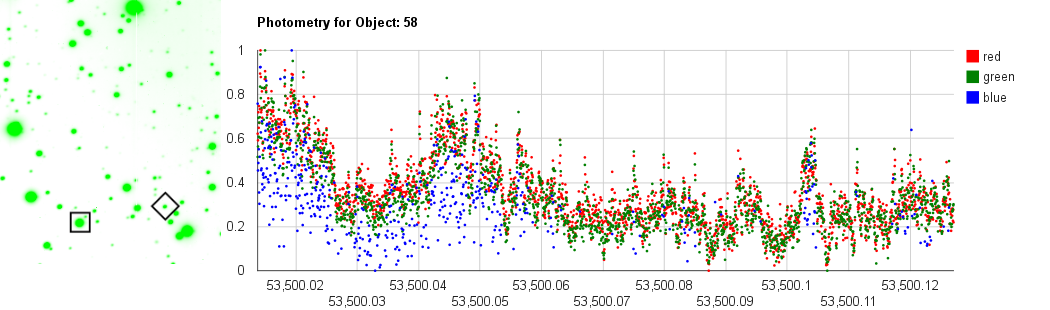
\includegraphics[width=150mm]{images/gumus-discovery-lc.png}
\caption{Flickering: A screen-capture from the web browser interface showing how variable objects reveal themselves when scrolling through the light-curves. The upper plot shows a non-variable object. The lower plot shows an object that is exhibiting flickering.  The currently-selected object is indicated by the diamond and the comparison object is indicated by the square. The y-axis of the light-curve is the relative flux of the selected object to the comparison object normalised to include the full range of variability within the same set of axes. The scaling of the y-axis was chosen to accentuate any variability in the light-curve and make it clearly visible in all three colours.}
\label{fig:gumus-discovery}
\end{figure}

\subsection{Exoplanet transit: KIC 511978}
The second example shows the detection of an exoplanet transit through inspection of the light-curves produced by the automated pipeline. The run \emph{2013-07-21/run010} was taken at the WHT in July as a follow up of KIC 5115978. This object is known to have at least one exoplanet, \citep{KIC5115978}. Although the transit does not have a large amplitude (approximately 1\% in relative flux), it is still clearly visible when browsing through the light-curves in the browser interface. 

\begin{figure}
\centering
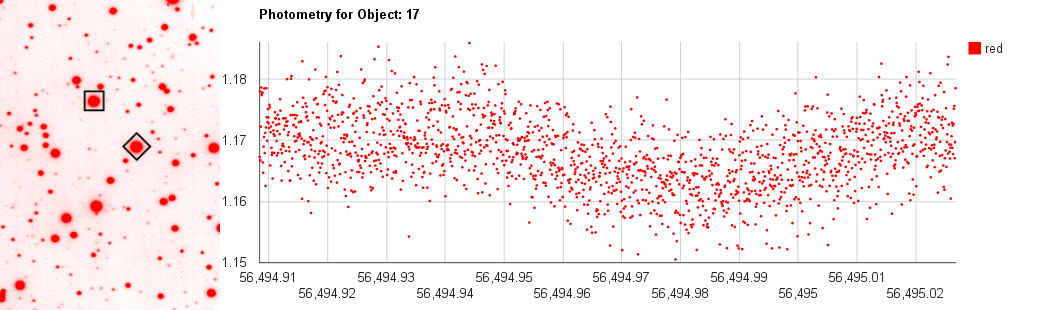
\includegraphics[width=150mm]{images/koi823-r-lc.png}
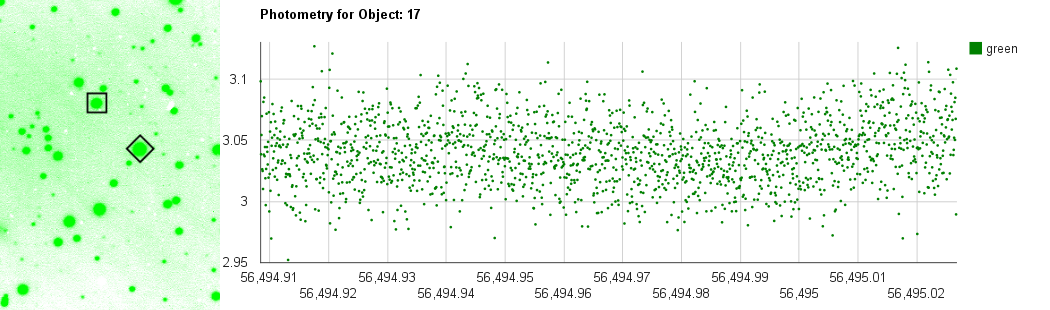
\includegraphics[width=150mm]{images/koi823-g-lc.png}
\caption{Exoplanet transit: A screen-capture from the web browser interface showing an exoplanet transit for KIC 5115978 in the Sloan i and g bands. The target object is indicated by the diamond and the comparison object is indicated by the square. The y-axis of the light-curve is the relative flux of the selected object to the comparison object.}
\label{fig:gumus-discovery}
\end{figure}

\subsection{Flare star: YZ CMi}
The third example shows how obvious a large change in the flux of a star is highlighted through the web browser. While scanning through the light-curves of this run \emph{2012-01-13/run015} a large increase was noted in for one of the objects. Looking at the observer's notes for the run, we saw that this was an observation of the flare star YZ Cmi. This is a particularly large flare with an increase of about 100 times in a narrow bandpass filter centred at 3500\AA, which is labeled `blue' in the web interface, figure \ref{fig:ultraflare-web}.  

\begin{figure}
\centering
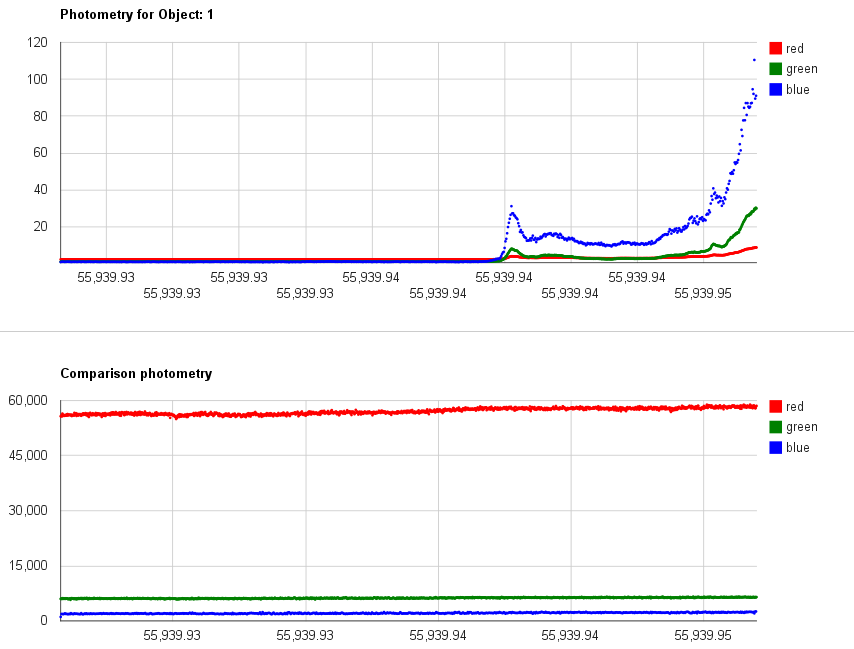
\includegraphics[width=150mm]{images/ultraflare-on-YZCMi.png}
\caption{Flare star: A large flare event noted in the web browser interface. This is the flare star YZ CMi undergoing a particularly dramatic flare event with its intensity increasing by a factor of 100 in the blue channel. The filters used for this run were two narrow band filters, centered at 3500\AA\  and 4170\AA\  for the blue and green channels and a red continuum filter centred at 6010\AA\  for the red channel. The star's intensity is plotted as its flux relative to the comparison star, shown in the lower plot. }
\label{fig:ultraflare-web}
\end{figure}


\section{Covering the entire ULTRACAM archive}
In order to make the processing of the ULTRACAM archive as free from manual intervention as possible, a few additional scripts were written to coordinate the steps of the pipeline as described in the previous two chapters. These wrapper scripts were designed to trigger the pipeline for a full night's set of observations with a single command. The University of Warwick has a high performance computing facility called `Cluster of Workstations' (CoWS) that uses idle computing time on all of the desktop machines in the department. A script was written that sends the automated pipeline processing jobs to this shared facility. Using this approach, it was possible to process nearly all of the ULTRACAM archive in about 2 weeks. At present, \emph{347} nights, out of a total of \emph{406}, have been processed and are available for viewing on a web server hosted at the University of Warwick. 

The runs that have not been processed are a few very high cadence runs with exposure times of less than 0.1 seconds and number of frames exceeding 50,000. The automated pipeline can take more than 8 hours processing time on these runs. The Cluster of Workstations has sufficient computing power to complete the processing task, however, it was felt that a different  and more optimised version of the pipeline should be built that will treat these runs differently. These runs usually contain very few objects, typically only the target object and a comparison and this situation is handled very well by the traditional pipeline. The processing of high cadence runs with very few objects was not a goal for this project. 

Of these 347 nights, approximately 20\% of the science runs have been investigated for objects with variability. The method of investigation is to perform a visual check of the light-curve. The web interface is designed such that it is easy for the viewer to examine the light-curves of all of the objects systematically. More information on how to use this interface can be found in the user manual, appendix \ref{chap:usermanual}. 

\section{Summary}
We have shown that the photometry produced by the automated pipeline is of sufficiently high quality to allow researchers to study the light-curves looking for and evaluating astronomical phenomena. Although our photometry is not calibrated, it is nevertheless useful for scientific purposes. Browsing through the ULTRACAM archive is quick and easy through the web browser interface which allows users to identify target objects by flipping through the light-curves. Other variable objects can be also discovered by recognising their variablility in the interface. The automated pipeline can cope with most of the diversity of data in the archive. It struggles with extremely high cadence runs and needs to be optimised to more reduce these data more efficiently.

In the next chapter we highlight a few objects that have been discovered using the automated pipeline. 
